% Options for packages loaded elsewhere
\PassOptionsToPackage{unicode}{hyperref}
\PassOptionsToPackage{hyphens}{url}
%
\documentclass[
]{article}
\usepackage{lmodern}
\usepackage{amssymb,amsmath}
\usepackage{ifxetex,ifluatex}
\ifnum 0\ifxetex 1\fi\ifluatex 1\fi=0 % if pdftex
  \usepackage[T1]{fontenc}
  \usepackage[utf8]{inputenc}
  \usepackage{textcomp} % provide euro and other symbols
\else % if luatex or xetex
  \usepackage{unicode-math}
  \defaultfontfeatures{Scale=MatchLowercase}
  \defaultfontfeatures[\rmfamily]{Ligatures=TeX,Scale=1}
\fi
% Use upquote if available, for straight quotes in verbatim environments
\IfFileExists{upquote.sty}{\usepackage{upquote}}{}
\IfFileExists{microtype.sty}{% use microtype if available
  \usepackage[]{microtype}
  \UseMicrotypeSet[protrusion]{basicmath} % disable protrusion for tt fonts
}{}
\makeatletter
\@ifundefined{KOMAClassName}{% if non-KOMA class
  \IfFileExists{parskip.sty}{%
    \usepackage{parskip}
  }{% else
    \setlength{\parindent}{0pt}
    \setlength{\parskip}{6pt plus 2pt minus 1pt}}
}{% if KOMA class
  \KOMAoptions{parskip=half}}
\makeatother
\usepackage{xcolor}
\IfFileExists{xurl.sty}{\usepackage{xurl}}{} % add URL line breaks if available
\IfFileExists{bookmark.sty}{\usepackage{bookmark}}{\usepackage{hyperref}}
\hypersetup{
  pdftitle={Exploratory Data Analysis},
  pdfauthor={Muhammad Ahsan},
  hidelinks,
  pdfcreator={LaTeX via pandoc}}
\urlstyle{same} % disable monospaced font for URLs
\usepackage[margin=1in]{geometry}
\usepackage{color}
\usepackage{fancyvrb}
\newcommand{\VerbBar}{|}
\newcommand{\VERB}{\Verb[commandchars=\\\{\}]}
\DefineVerbatimEnvironment{Highlighting}{Verbatim}{commandchars=\\\{\}}
% Add ',fontsize=\small' for more characters per line
\usepackage{framed}
\definecolor{shadecolor}{RGB}{248,248,248}
\newenvironment{Shaded}{\begin{snugshade}}{\end{snugshade}}
\newcommand{\AlertTok}[1]{\textcolor[rgb]{0.94,0.16,0.16}{#1}}
\newcommand{\AnnotationTok}[1]{\textcolor[rgb]{0.56,0.35,0.01}{\textbf{\textit{#1}}}}
\newcommand{\AttributeTok}[1]{\textcolor[rgb]{0.77,0.63,0.00}{#1}}
\newcommand{\BaseNTok}[1]{\textcolor[rgb]{0.00,0.00,0.81}{#1}}
\newcommand{\BuiltInTok}[1]{#1}
\newcommand{\CharTok}[1]{\textcolor[rgb]{0.31,0.60,0.02}{#1}}
\newcommand{\CommentTok}[1]{\textcolor[rgb]{0.56,0.35,0.01}{\textit{#1}}}
\newcommand{\CommentVarTok}[1]{\textcolor[rgb]{0.56,0.35,0.01}{\textbf{\textit{#1}}}}
\newcommand{\ConstantTok}[1]{\textcolor[rgb]{0.00,0.00,0.00}{#1}}
\newcommand{\ControlFlowTok}[1]{\textcolor[rgb]{0.13,0.29,0.53}{\textbf{#1}}}
\newcommand{\DataTypeTok}[1]{\textcolor[rgb]{0.13,0.29,0.53}{#1}}
\newcommand{\DecValTok}[1]{\textcolor[rgb]{0.00,0.00,0.81}{#1}}
\newcommand{\DocumentationTok}[1]{\textcolor[rgb]{0.56,0.35,0.01}{\textbf{\textit{#1}}}}
\newcommand{\ErrorTok}[1]{\textcolor[rgb]{0.64,0.00,0.00}{\textbf{#1}}}
\newcommand{\ExtensionTok}[1]{#1}
\newcommand{\FloatTok}[1]{\textcolor[rgb]{0.00,0.00,0.81}{#1}}
\newcommand{\FunctionTok}[1]{\textcolor[rgb]{0.00,0.00,0.00}{#1}}
\newcommand{\ImportTok}[1]{#1}
\newcommand{\InformationTok}[1]{\textcolor[rgb]{0.56,0.35,0.01}{\textbf{\textit{#1}}}}
\newcommand{\KeywordTok}[1]{\textcolor[rgb]{0.13,0.29,0.53}{\textbf{#1}}}
\newcommand{\NormalTok}[1]{#1}
\newcommand{\OperatorTok}[1]{\textcolor[rgb]{0.81,0.36,0.00}{\textbf{#1}}}
\newcommand{\OtherTok}[1]{\textcolor[rgb]{0.56,0.35,0.01}{#1}}
\newcommand{\PreprocessorTok}[1]{\textcolor[rgb]{0.56,0.35,0.01}{\textit{#1}}}
\newcommand{\RegionMarkerTok}[1]{#1}
\newcommand{\SpecialCharTok}[1]{\textcolor[rgb]{0.00,0.00,0.00}{#1}}
\newcommand{\SpecialStringTok}[1]{\textcolor[rgb]{0.31,0.60,0.02}{#1}}
\newcommand{\StringTok}[1]{\textcolor[rgb]{0.31,0.60,0.02}{#1}}
\newcommand{\VariableTok}[1]{\textcolor[rgb]{0.00,0.00,0.00}{#1}}
\newcommand{\VerbatimStringTok}[1]{\textcolor[rgb]{0.31,0.60,0.02}{#1}}
\newcommand{\WarningTok}[1]{\textcolor[rgb]{0.56,0.35,0.01}{\textbf{\textit{#1}}}}
\usepackage{graphicx,grffile}
\makeatletter
\def\maxwidth{\ifdim\Gin@nat@width>\linewidth\linewidth\else\Gin@nat@width\fi}
\def\maxheight{\ifdim\Gin@nat@height>\textheight\textheight\else\Gin@nat@height\fi}
\makeatother
% Scale images if necessary, so that they will not overflow the page
% margins by default, and it is still possible to overwrite the defaults
% using explicit options in \includegraphics[width, height, ...]{}
\setkeys{Gin}{width=\maxwidth,height=\maxheight,keepaspectratio}
% Set default figure placement to htbp
\makeatletter
\def\fps@figure{htbp}
\makeatother
\setlength{\emergencystretch}{3em} % prevent overfull lines
\providecommand{\tightlist}{%
  \setlength{\itemsep}{0pt}\setlength{\parskip}{0pt}}
\setcounter{secnumdepth}{-\maxdimen} % remove section numbering
% https://github.com/rstudio/rmarkdown/issues/337
\let\rmarkdownfootnote\footnote%
\def\footnote{\protect\rmarkdownfootnote}

% https://github.com/rstudio/rmarkdown/pull/252
\usepackage{titling}
\setlength{\droptitle}{-2em}

\pretitle{\vspace{\droptitle}\centering\huge}
\posttitle{\par}

\preauthor{\centering\large\emph}
\postauthor{\par}

\predate{\centering\large\emph}
\postdate{\par}

\title{Exploratory Data Analysis}
\author{Muhammad Ahsan}
\date{}

\begin{document}
\maketitle

\hypertarget{cardio-fitness-project}{%
\subsection{Cardio Fitness Project}\label{cardio-fitness-project}}

\hypertarget{project-objective}{%
\subsubsection{1. Project Objective}\label{project-objective}}

The objective of the report is to explore the cardio data set
(“CardioGoodFitness”) in R and generate insights about the data set.
This exploration report will consists of the following:

\begin{enumerate}
\def\labelenumi{\arabic{enumi}.}
\tightlist
\item
  Importing the dataset in R\\
\item
  Understanding the structure of dataset\\
\item
  Graphical exploration\\
\item
  Descriptive statistics\\
\item
  Insights from the dataset
\end{enumerate}

\hypertarget{assumptions}{%
\subsubsection{2. Assumptions}\label{assumptions}}

we assume data has normally distribution its mean the graph of the data
has a bell curve or skewed.data is independent and it has linear
relationship.we will do the further analysis to prove our assumstion.

\hypertarget{exploratory-data-analysis-uxe2-step-by-step-approach}{%
\subsubsection{3. Exploratory Data Analysis – Step by step
approach}\label{exploratory-data-analysis-uxe2-step-by-step-approach}}

A Typical Data exploration activity consists of the following steps:

\hypertarget{environment-set-up-and-data-import}{%
\paragraph{3.1 Environment Set up and Data
Import}\label{environment-set-up-and-data-import}}

\hypertarget{required-libraries}{%
\paragraph{Required Libraries}\label{required-libraries}}

\begin{Shaded}
\begin{Highlighting}[]
\CommentTok{#library(readr)}
\KeywordTok{library}\NormalTok{(ggplot2)}
\KeywordTok{library}\NormalTok{(gridExtra)}
\KeywordTok{library}\NormalTok{(corrplot)}
\KeywordTok{library}\NormalTok{(scales)}
\end{Highlighting}
\end{Shaded}

\hypertarget{setting-up-working-directory-and-importing-the-dataset}{%
\subparagraph{Setting up working Directory and importing the
Dataset}\label{setting-up-working-directory-and-importing-the-dataset}}

In this chunk we set the working directory and importing the dataset for
analysis and we convert the dataset in Data Frames

\begin{Shaded}
\begin{Highlighting}[]
\KeywordTok{setwd}\NormalTok{(}\StringTok{"C:/Users/AHSAN/Documents/R-cardio-data-analysis-project-"}\NormalTok{)}
\NormalTok{cardio_data <-}\StringTok{ }\KeywordTok{read.csv}\NormalTok{(}\StringTok{"CardioGoodFitness.csv"}\NormalTok{)}
\NormalTok{cardio_data <-}\StringTok{ }\KeywordTok{data.frame}\NormalTok{(cardio_data)}
\end{Highlighting}
\end{Shaded}

\hypertarget{variable-identification}{%
\paragraph{3.2 Variable Identification}\label{variable-identification}}

we are using ``dim()'' function to get the dimention or shape of the
dataset. ``names()'' this function we going to use is getting the names
or columns of the dataset. ``head()'' this function is use for
presenting top some rows or observations of the dataset bydefault we ill
get top 5 rows but we can add specific also." ``tail()'' retun the last
5 rows by default

\#\#\#\#dimention of the dataset

\begin{Shaded}
\begin{Highlighting}[]
\KeywordTok{dim}\NormalTok{(cardio_data)}
\end{Highlighting}
\end{Shaded}

\begin{verbatim}
## [1] 180   9
\end{verbatim}

This data set has 180 observation and 9 veriables/columns.

\#\#\#\#Columns of the dataset

\begin{Shaded}
\begin{Highlighting}[]
\KeywordTok{names}\NormalTok{(cardio_data)}
\end{Highlighting}
\end{Shaded}

\begin{verbatim}
## [1] "Product"       "Age"           "Gender"        "Education"    
## [5] "MaritalStatus" "Usage"         "Fitness"       "Income"       
## [9] "Miles"
\end{verbatim}

\#\#\#\#Structure of the dataset

\begin{Shaded}
\begin{Highlighting}[]
\KeywordTok{str}\NormalTok{(cardio_data)}
\end{Highlighting}
\end{Shaded}

\begin{verbatim}
## 'data.frame':    180 obs. of  9 variables:
##  $ Product      : Factor w/ 3 levels "TM195","TM498",..: 1 1 1 1 1 1 1 1 1 1 ...
##  $ Age          : int  18 19 19 19 20 20 21 21 21 21 ...
##  $ Gender       : Factor w/ 2 levels "Female","Male": 2 2 1 2 2 1 1 2 2 1 ...
##  $ Education    : int  14 15 14 12 13 14 14 13 15 15 ...
##  $ MaritalStatus: Factor w/ 2 levels "Partnered","Single": 2 2 1 2 1 1 1 2 2 1 ...
##  $ Usage        : int  3 2 4 3 4 3 3 3 5 2 ...
##  $ Fitness      : int  4 3 3 3 2 3 3 3 4 3 ...
##  $ Income       : int  29562 31836 30699 32973 35247 32973 35247 32973 35247 37521 ...
##  $ Miles        : int  112 75 66 85 47 66 75 85 141 85 ...
\end{verbatim}

\#\#\#\#Top 5 rows of the dataset

\begin{Shaded}
\begin{Highlighting}[]
\KeywordTok{head}\NormalTok{(cardio_data)}
\end{Highlighting}
\end{Shaded}

\begin{verbatim}
##   Product Age Gender Education MaritalStatus Usage Fitness Income Miles
## 1   TM195  18   Male        14        Single     3       4  29562   112
## 2   TM195  19   Male        15        Single     2       3  31836    75
## 3   TM195  19 Female        14     Partnered     4       3  30699    66
## 4   TM195  19   Male        12        Single     3       3  32973    85
## 5   TM195  20   Male        13     Partnered     4       2  35247    47
## 6   TM195  20 Female        14     Partnered     3       3  32973    66
\end{verbatim}

\#\#\#\#Last 5 rows of the dataset

\begin{Shaded}
\begin{Highlighting}[]
\KeywordTok{tail}\NormalTok{(cardio_data)}
\end{Highlighting}
\end{Shaded}

\begin{verbatim}
##     Product Age Gender Education MaritalStatus Usage Fitness Income Miles
## 175   TM798  38   Male        18     Partnered     5       5 104581   150
## 176   TM798  40   Male        21        Single     6       5  83416   200
## 177   TM798  42   Male        18        Single     5       4  89641   200
## 178   TM798  45   Male        16        Single     5       5  90886   160
## 179   TM798  47   Male        18     Partnered     4       5 104581   120
## 180   TM798  48   Male        18     Partnered     4       5  95508   180
\end{verbatim}

\#\#\#\#Convertion of some columns datatype cracter to factor

\begin{Shaded}
\begin{Highlighting}[]
\NormalTok{cardio_data}\OperatorTok{$}\NormalTok{Product <-}\StringTok{ }\KeywordTok{as.factor}\NormalTok{(cardio_data}\OperatorTok{$}\NormalTok{Product)}
\NormalTok{cardio_data}\OperatorTok{$}\NormalTok{Gender <-}\StringTok{ }\KeywordTok{as.factor}\NormalTok{(cardio_data}\OperatorTok{$}\NormalTok{Gender)}
\NormalTok{cardio_data}\OperatorTok{$}\NormalTok{MaritalStatus <-}\StringTok{ }\KeywordTok{as.factor}\NormalTok{(cardio_data}\OperatorTok{$}\NormalTok{MaritalStatus)}
\NormalTok{cardio_data}\OperatorTok{$}\NormalTok{Education <-}\StringTok{ }\KeywordTok{as.factor}\NormalTok{(cardio_data}\OperatorTok{$}\NormalTok{Education)}
\end{Highlighting}
\end{Shaded}

\#\#\#\#Summary of the data

\begin{Shaded}
\begin{Highlighting}[]
\CommentTok{#Statisticl Summary of Dataset}
\KeywordTok{summary}\NormalTok{(cardio_data)}
\end{Highlighting}
\end{Shaded}

\begin{verbatim}
##   Product        Age           Gender      Education    MaritalStatus
##  TM195:80   Min.   :18.00   Female: 76   16     :85   Partnered:107  
##  TM498:60   1st Qu.:24.00   Male  :104   14     :55   Single   : 73  
##  TM798:40   Median :26.00                18     :23                  
##             Mean   :28.79                13     : 5                  
##             3rd Qu.:33.00                15     : 5                  
##             Max.   :50.00                12     : 3                  
##                                          (Other): 4                  
##      Usage          Fitness          Income           Miles      
##  Min.   :2.000   Min.   :1.000   Min.   : 29562   Min.   : 21.0  
##  1st Qu.:3.000   1st Qu.:3.000   1st Qu.: 44059   1st Qu.: 66.0  
##  Median :3.000   Median :3.000   Median : 50597   Median : 94.0  
##  Mean   :3.456   Mean   :3.311   Mean   : 53720   Mean   :103.2  
##  3rd Qu.:4.000   3rd Qu.:4.000   3rd Qu.: 58668   3rd Qu.:114.8  
##  Max.   :7.000   Max.   :5.000   Max.   :104581   Max.   :360.0  
## 
\end{verbatim}

statistical summary tell us the minimum,first qrartile,median, third
quartile and maximum value of the dataset.

\hypertarget{univariate-analysis}{%
\subsubsection{3.3 Univariate Analysis}\label{univariate-analysis}}

Univerable analysis is using for single or uni veriable of the dataset
we also check how veriable is distributed.

\#\#\#\#Products summary and plot:

\begin{Shaded}
\begin{Highlighting}[]
\CommentTok{#Statisticl Summary of Product }
\KeywordTok{summary}\NormalTok{(cardio_data}\OperatorTok{$}\NormalTok{Product)}
\end{Highlighting}
\end{Shaded}

\begin{verbatim}
## TM195 TM498 TM798 
##    80    60    40
\end{verbatim}

\begin{Shaded}
\begin{Highlighting}[]
\CommentTok{#product plot }
\NormalTok{p<-}\StringTok{ }\KeywordTok{ggplot}\NormalTok{(}\DataTypeTok{data =}\NormalTok{ cardio_data, }\KeywordTok{aes}\NormalTok{(}\DataTypeTok{x =}\NormalTok{ Product)) }\OperatorTok{+}\StringTok{ }
\StringTok{  }\KeywordTok{geom_bar}\NormalTok{(}\DataTypeTok{color=}\StringTok{"black"}\NormalTok{ ,}\DataTypeTok{fill=}\StringTok{"darkcyan"}\NormalTok{) }\OperatorTok{+}
\StringTok{  }\KeywordTok{theme_grey}\NormalTok{() }\OperatorTok{+}\StringTok{ }\KeywordTok{ggtitle}\NormalTok{(}\StringTok{"Product Plot    fig-(1.1)"}\NormalTok{)}\OperatorTok{+}\KeywordTok{xlab}\NormalTok{(}\StringTok{"Product"}\NormalTok{)}\OperatorTok{+}
\StringTok{  }\KeywordTok{geom_text}\NormalTok{(}\DataTypeTok{stat =} \StringTok{'count'}\NormalTok{,}\KeywordTok{aes}\NormalTok{(}\DataTypeTok{label =}\NormalTok{..count.., }\DataTypeTok{vjust =} \FloatTok{-0.2}\NormalTok{))}
\NormalTok{p}
\end{Highlighting}
\end{Shaded}

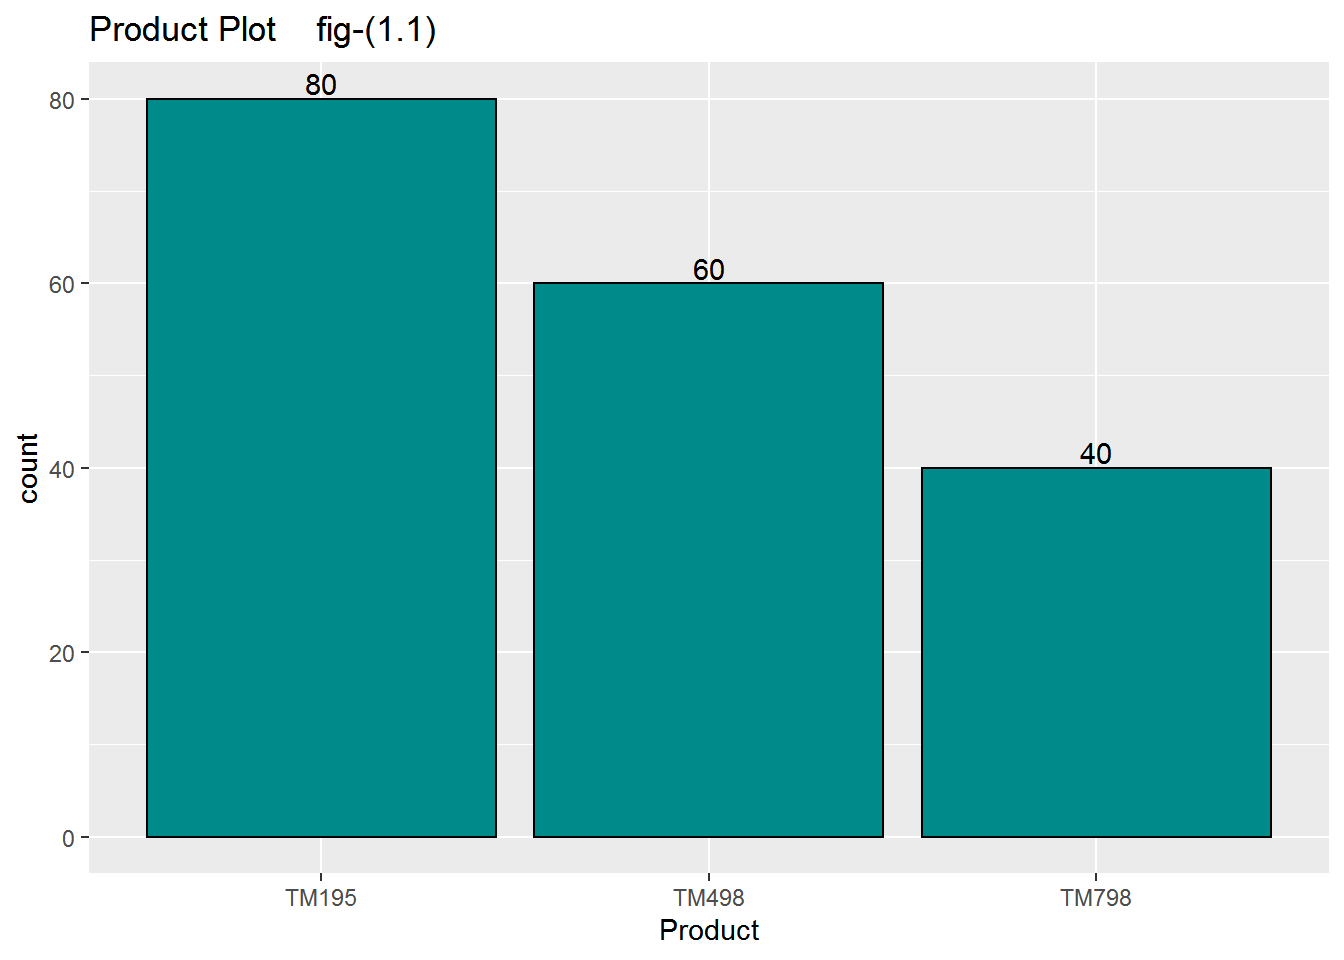
\includegraphics{index_files/figure-latex/unnamed-chunk-10-1.pdf}

as we saw in this graph fig(1.1) we have three products in this dataset
one name is TM195,2ND TM498, 3RD TM798. TM195 give us the highest number
of count its mean the dataset provided us most of the user using Tm 195
treadmill then Tm498 then tm 798 respectively.

\#\#\#\#Age,Education and Usage sumary and plots

\begin{Shaded}
\begin{Highlighting}[]
\CommentTok{#Statisticl Summary of Age}
\KeywordTok{summary}\NormalTok{(cardio_data}\OperatorTok{$}\NormalTok{Age)}
\end{Highlighting}
\end{Shaded}

\begin{verbatim}
##    Min. 1st Qu.  Median    Mean 3rd Qu.    Max. 
##   18.00   24.00   26.00   28.79   33.00   50.00
\end{verbatim}

\begin{Shaded}
\begin{Highlighting}[]
\KeywordTok{sd}\NormalTok{(cardio_data}\OperatorTok{$}\NormalTok{Age)}
\end{Highlighting}
\end{Shaded}

\begin{verbatim}
## [1] 6.943498
\end{verbatim}

\begin{Shaded}
\begin{Highlighting}[]
\CommentTok{#ge plot }
\NormalTok{p1<-}\StringTok{ }\KeywordTok{ggplot}\NormalTok{(}\DataTypeTok{data =}\NormalTok{ cardio_data, }\KeywordTok{aes}\NormalTok{(}\DataTypeTok{x =}\NormalTok{ Age)) }\OperatorTok{+}\StringTok{ }
\StringTok{  }\KeywordTok{geom_histogram}\NormalTok{(}\DataTypeTok{bins =} \DecValTok{30}\NormalTok{, }\DataTypeTok{color=}\StringTok{"black"}\NormalTok{ ,}\DataTypeTok{fill=}\StringTok{"darkcyan"}\NormalTok{) }\OperatorTok{+}
\StringTok{  }\KeywordTok{theme_grey}\NormalTok{() }\OperatorTok{+}\StringTok{ }\KeywordTok{ggtitle}\NormalTok{(}\StringTok{"Histogram of Age"}\NormalTok{)}\OperatorTok{+}\KeywordTok{xlab}\NormalTok{(}\StringTok{"Age (Years)"}\NormalTok{)}
\CommentTok{#Statisticl Summary of education}
\KeywordTok{summary}\NormalTok{(cardio_data}\OperatorTok{$}\NormalTok{Education)}
\end{Highlighting}
\end{Shaded}

\begin{verbatim}
## 12 13 14 15 16 18 20 21 
##  3  5 55  5 85 23  1  3
\end{verbatim}

\begin{Shaded}
\begin{Highlighting}[]
\CommentTok{#education plot }
\NormalTok{p2<-}\KeywordTok{ggplot}\NormalTok{(}\DataTypeTok{data =}\NormalTok{ cardio_data, }\KeywordTok{aes}\NormalTok{(}\DataTypeTok{x =}\NormalTok{ Education)) }\OperatorTok{+}\StringTok{ }
\StringTok{  }\KeywordTok{geom_bar}\NormalTok{(}\DataTypeTok{color=}\StringTok{"black"}\NormalTok{ ,}\DataTypeTok{fill=}\StringTok{"darkcyan"}\NormalTok{) }\OperatorTok{+}
\StringTok{  }\KeywordTok{theme_grey}\NormalTok{() }\OperatorTok{+}\StringTok{ }\KeywordTok{ggtitle}\NormalTok{(}\StringTok{" Education Bar plot "}\NormalTok{)}\OperatorTok{+}
\StringTok{  }\KeywordTok{geom_text}\NormalTok{(}\DataTypeTok{stat =} \StringTok{'count'}\NormalTok{,}\KeywordTok{aes}\NormalTok{(}\DataTypeTok{label =}\NormalTok{..count.., }\DataTypeTok{vjust =} \FloatTok{-0.2}\NormalTok{))}
\CommentTok{#Statisticl Summary of usage}
\KeywordTok{summary}\NormalTok{(cardio_data}\OperatorTok{$}\NormalTok{Usage)}
\end{Highlighting}
\end{Shaded}

\begin{verbatim}
##    Min. 1st Qu.  Median    Mean 3rd Qu.    Max. 
##   2.000   3.000   3.000   3.456   4.000   7.000
\end{verbatim}

\begin{Shaded}
\begin{Highlighting}[]
\CommentTok{#usage plot }
\NormalTok{p3<-}\KeywordTok{ggplot}\NormalTok{(}\DataTypeTok{data =}\NormalTok{ cardio_data, }\KeywordTok{aes}\NormalTok{(}\DataTypeTok{x =}\NormalTok{ Usage)) }\OperatorTok{+}\StringTok{ }
\StringTok{  }\KeywordTok{geom_bar}\NormalTok{(}\DataTypeTok{color=}\StringTok{"black"}\NormalTok{ ,}\DataTypeTok{fill=}\StringTok{"darkcyan"}\NormalTok{) }\OperatorTok{+}
\StringTok{  }\KeywordTok{theme_grey}\NormalTok{() }\OperatorTok{+}\StringTok{ }\KeywordTok{ggtitle}\NormalTok{(}\StringTok{" Usage of Machines "}\NormalTok{)}\OperatorTok{+}
\StringTok{  }\KeywordTok{geom_text}\NormalTok{(}\DataTypeTok{stat =} \StringTok{'count'}\NormalTok{,}\KeywordTok{aes}\NormalTok{(}\DataTypeTok{label =}\KeywordTok{percent}\NormalTok{(}\KeywordTok{round}\NormalTok{(..count..}\OperatorTok{/}\KeywordTok{length}\NormalTok{(cardio_data}\OperatorTok{$}\NormalTok{Usage),}\DecValTok{4}\NormalTok{)), }\DataTypeTok{vjust =} \FloatTok{-0.3}\NormalTok{))}
\CommentTok{#combining the plots}
\KeywordTok{grid.arrange}\NormalTok{(p1,p2,p3,}\DataTypeTok{ncol=}\DecValTok{3}\NormalTok{)}
\end{Highlighting}
\end{Shaded}

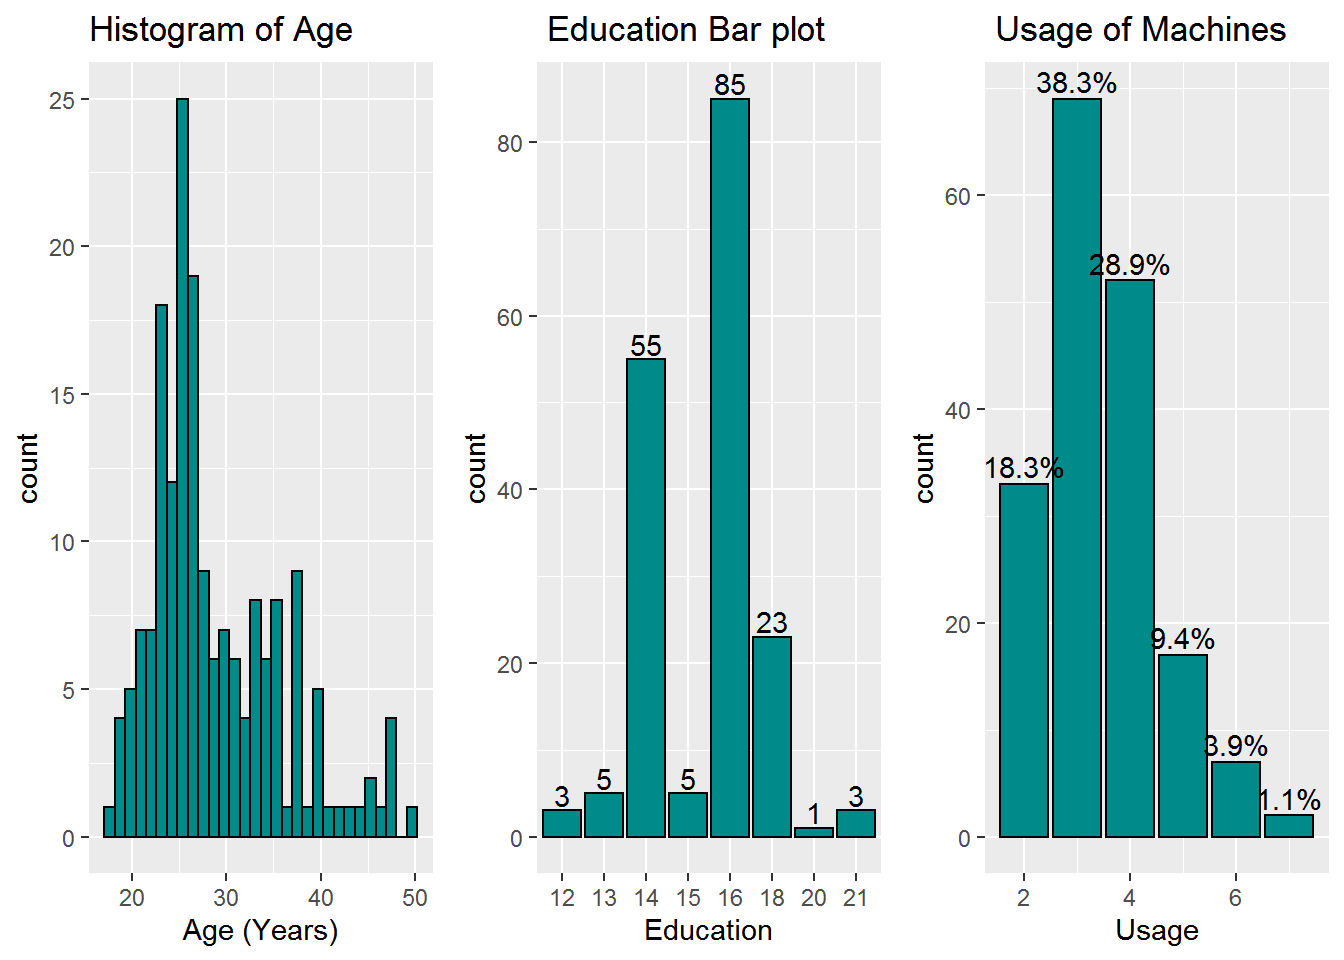
\includegraphics{index_files/figure-latex/unnamed-chunk-11-1.pdf}

if we saw the summary of the age, mean is slightly higher then the
median and the distrubtion of the age is right skwed.if we find the
coefficient of variation we only have 24\%. its tell us sample age is
not equally distributed. 2nd towards education plot its tell us the data
sample people mostly are the 16 years of education it has 85 counts. 3rd
usage of treadmill mostly user use the traedmill 38\% of the people
using the treadmill three times a week 29\% of the people using 4 times
a week.18\% using only two times.

\hypertarget{gender-summary-and-plot}{%
\paragraph{Gender summary and plot}\label{gender-summary-and-plot}}

\begin{Shaded}
\begin{Highlighting}[]
\CommentTok{#Statisticl Summary of Gender}
\KeywordTok{summary}\NormalTok{(cardio_data}\OperatorTok{$}\NormalTok{Gender)}
\end{Highlighting}
\end{Shaded}

\begin{verbatim}
## Female   Male 
##     76    104
\end{verbatim}

\begin{Shaded}
\begin{Highlighting}[]
\KeywordTok{ggplot}\NormalTok{(}\DataTypeTok{data =}\NormalTok{ cardio_data, }\KeywordTok{aes}\NormalTok{(}\DataTypeTok{x =}\NormalTok{ Gender)) }\OperatorTok{+}\StringTok{ }
\StringTok{  }\KeywordTok{geom_bar}\NormalTok{(}\DataTypeTok{color=}\StringTok{"black"}\NormalTok{ ,}\DataTypeTok{fill=}\StringTok{"darkcyan"}\NormalTok{) }\OperatorTok{+}
\StringTok{  }\KeywordTok{theme_grey}\NormalTok{() }\OperatorTok{+}\StringTok{ }\KeywordTok{ggtitle}\NormalTok{(}\StringTok{"Gender Ploting"}\NormalTok{)}\OperatorTok{+}
\StringTok{  }\KeywordTok{geom_text}\NormalTok{(}\DataTypeTok{stat =} \StringTok{'count'}\NormalTok{,}\KeywordTok{aes}\NormalTok{(}\DataTypeTok{label =}\NormalTok{..count.., }\DataTypeTok{vjust =} \FloatTok{-0.2}\NormalTok{))}
\end{Highlighting}
\end{Shaded}

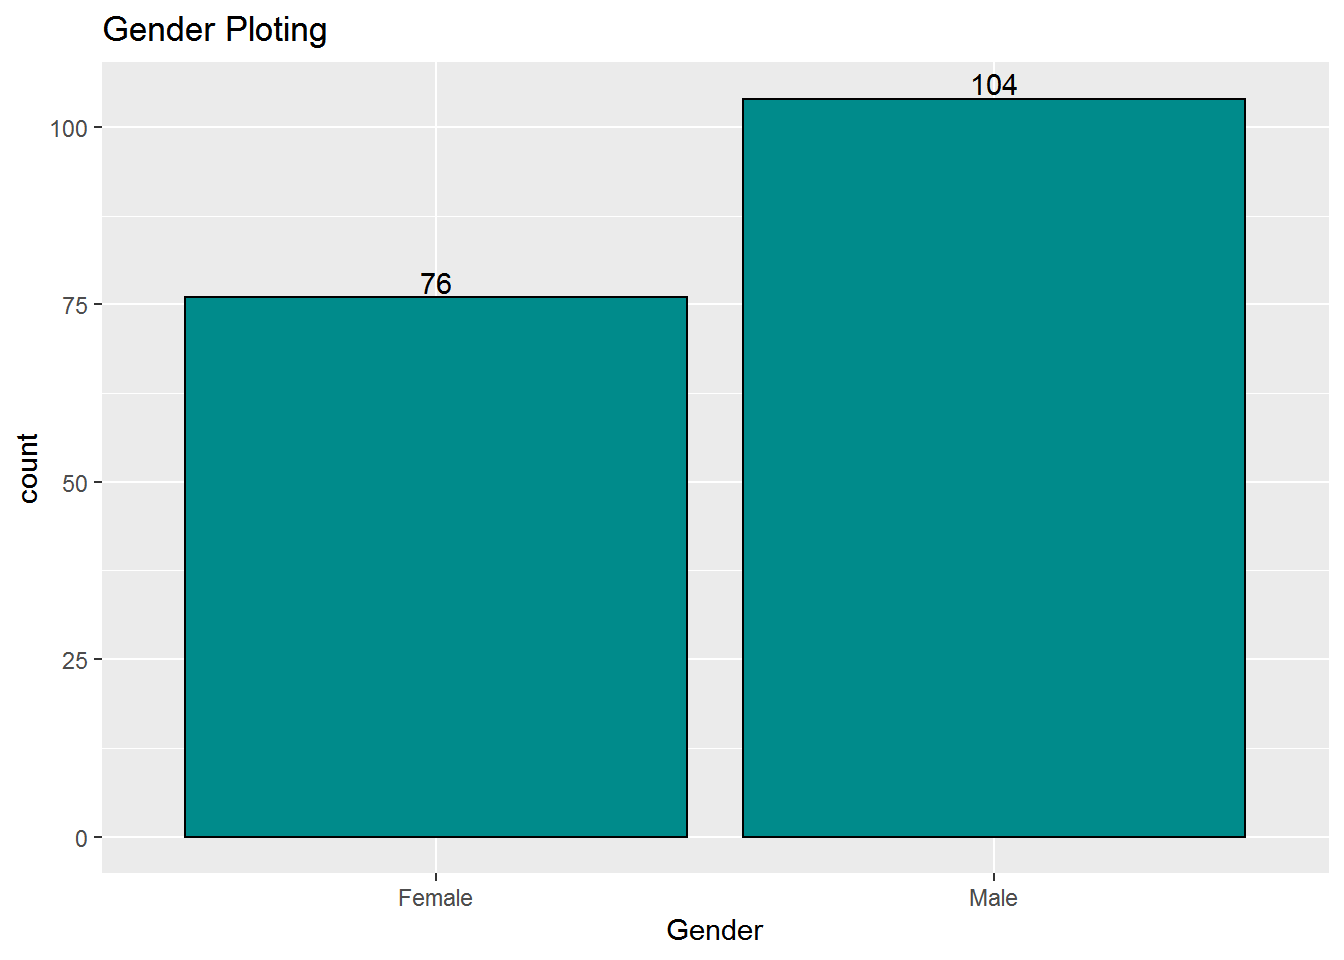
\includegraphics{index_files/figure-latex/unnamed-chunk-12-1.pdf}

in this ploting the no of male users are 104 and female users are 76.

\#\#\#\#Marital status and income summary and plot

\begin{Shaded}
\begin{Highlighting}[]
\CommentTok{#Statisticl Summary of Marital Status}
\KeywordTok{summary}\NormalTok{(cardio_data}\OperatorTok{$}\NormalTok{MaritalStatus)}
\end{Highlighting}
\end{Shaded}

\begin{verbatim}
## Partnered    Single 
##       107        73
\end{verbatim}

\begin{Shaded}
\begin{Highlighting}[]
\CommentTok{#Maritel status plot }
\NormalTok{p1<-}\StringTok{ }\KeywordTok{ggplot}\NormalTok{(}\DataTypeTok{data =}\NormalTok{ cardio_data, }\KeywordTok{aes}\NormalTok{(}\DataTypeTok{x =}\NormalTok{ MaritalStatus)) }\OperatorTok{+}\StringTok{ }
\StringTok{  }\KeywordTok{geom_bar}\NormalTok{( }\DataTypeTok{color=}\StringTok{"black"}\NormalTok{ ,}\DataTypeTok{fill=}\StringTok{"darkcyan"}\NormalTok{) }\OperatorTok{+}
\StringTok{  }\KeywordTok{theme_grey}\NormalTok{() }\OperatorTok{+}\StringTok{ }\KeywordTok{ggtitle}\NormalTok{(}\StringTok{"User Marital Status"}\NormalTok{)}\OperatorTok{+}
\StringTok{  }\KeywordTok{geom_text}\NormalTok{(}\DataTypeTok{stat =} \StringTok{'count'}\NormalTok{,}\KeywordTok{aes}\NormalTok{(}\DataTypeTok{label =}\NormalTok{..count.., }\DataTypeTok{vjust =} \FloatTok{-0.2}\NormalTok{))}
\CommentTok{#Statisticl Summary of income}
\KeywordTok{summary}\NormalTok{(cardio_data}\OperatorTok{$}\NormalTok{Income)}
\end{Highlighting}
\end{Shaded}

\begin{verbatim}
##    Min. 1st Qu.  Median    Mean 3rd Qu.    Max. 
##   29562   44059   50597   53720   58668  104581
\end{verbatim}

\begin{Shaded}
\begin{Highlighting}[]
\KeywordTok{sd}\NormalTok{(cardio_data}\OperatorTok{$}\NormalTok{Income)}
\end{Highlighting}
\end{Shaded}

\begin{verbatim}
## [1] 16506.68
\end{verbatim}

\begin{Shaded}
\begin{Highlighting}[]
\CommentTok{#Income plot}
\NormalTok{p2<-}\StringTok{ }\KeywordTok{ggplot}\NormalTok{(}\DataTypeTok{data =}\NormalTok{ cardio_data, }\KeywordTok{aes}\NormalTok{(}\DataTypeTok{x =}\NormalTok{ Income)) }\OperatorTok{+}\StringTok{ }
\StringTok{  }\KeywordTok{geom_histogram}\NormalTok{(}\DataTypeTok{bins =} \DecValTok{50}\NormalTok{, }\DataTypeTok{color=}\StringTok{"black"}\NormalTok{ ,}\DataTypeTok{fill=}\StringTok{"darkcyan"}\NormalTok{) }\OperatorTok{+}
\StringTok{  }\KeywordTok{theme_grey}\NormalTok{() }\OperatorTok{+}\StringTok{ }\KeywordTok{scale_x_continuous}\NormalTok{(}\DataTypeTok{labels =}\NormalTok{ scales}\OperatorTok{::}\NormalTok{comma) }\OperatorTok{+}\StringTok{ }\KeywordTok{ggtitle}\NormalTok{(}\StringTok{"Histogram Of User Income"}\NormalTok{)}


\NormalTok{p3<-}\StringTok{ }\KeywordTok{ggplot}\NormalTok{(}\DataTypeTok{data =}\NormalTok{ cardio_data, }\KeywordTok{aes}\NormalTok{(}\DataTypeTok{x =} \StringTok{""}\NormalTok{,}\DataTypeTok{y=}\NormalTok{Income)) }\OperatorTok{+}\StringTok{ }
\StringTok{  }\KeywordTok{geom_boxplot}\NormalTok{(}\DataTypeTok{color=}\StringTok{"black"}\NormalTok{ ,}\DataTypeTok{fill=}\StringTok{"darkcyan"}\NormalTok{) }\OperatorTok{+}
\StringTok{  }\KeywordTok{theme_grey}\NormalTok{() }\OperatorTok{+}\StringTok{  }\KeywordTok{ggtitle}\NormalTok{(}\StringTok{"User Income"}\NormalTok{)}\OperatorTok{+}\StringTok{ }\KeywordTok{scale_y_continuous}\NormalTok{(}\DataTypeTok{labels =}\NormalTok{ scales}\OperatorTok{::}\NormalTok{comma) }
\CommentTok{#combining the plots}
\KeywordTok{grid.arrange}\NormalTok{(p1,p2,p3,}\DataTypeTok{ncol=}\DecValTok{3}\NormalTok{)}
\end{Highlighting}
\end{Shaded}

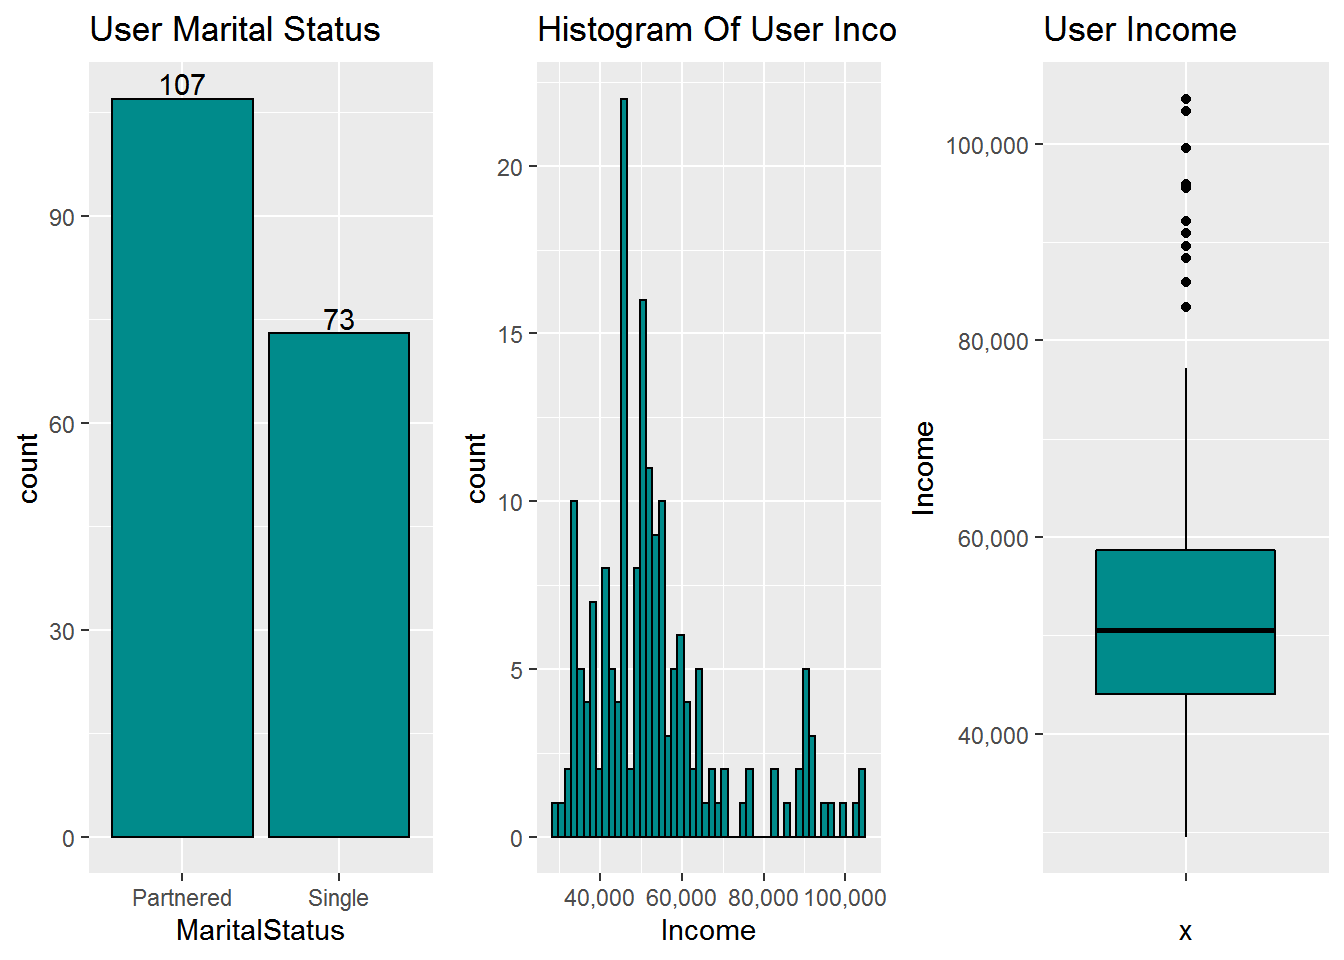
\includegraphics{index_files/figure-latex/unnamed-chunk-13-1.pdf}

107 member has a partenered and 73 persons are single.user income has
right skwed distribution because the mean is greater then median and
coefficient of variation is 30\%.

\hypertarget{bivariate-analysis}{%
\subsubsection{3.4 bivariate Analysis}\label{bivariate-analysis}}

\begin{Shaded}
\begin{Highlighting}[]
\CommentTok{#statistical summary of Age and Gender}
\KeywordTok{tapply}\NormalTok{(cardio_data}\OperatorTok{$}\NormalTok{Age,cardio_data}\OperatorTok{$}\NormalTok{Gender,summary)}
\end{Highlighting}
\end{Shaded}

\begin{verbatim}
## $Female
##    Min. 1st Qu.  Median    Mean 3rd Qu.    Max. 
##   19.00   24.00   26.50   28.57   33.00   50.00 
## 
## $Male
##    Min. 1st Qu.  Median    Mean 3rd Qu.    Max. 
##   18.00   23.75   26.00   28.95   34.00   48.00
\end{verbatim}

\begin{Shaded}
\begin{Highlighting}[]
\KeywordTok{ggplot}\NormalTok{(cardio_data,}\KeywordTok{aes}\NormalTok{(}\DataTypeTok{x=}\NormalTok{ Gender,}\DataTypeTok{y=}\NormalTok{Age)) }\OperatorTok{+}\KeywordTok{geom_boxplot}\NormalTok{(}\KeywordTok{aes}\NormalTok{(}\DataTypeTok{colour =}\NormalTok{ Gender), }\DataTypeTok{outlier.colour =} \StringTok{"red"}\NormalTok{,}\DataTypeTok{notch=}\OtherTok{TRUE}\NormalTok{) }
\end{Highlighting}
\end{Shaded}

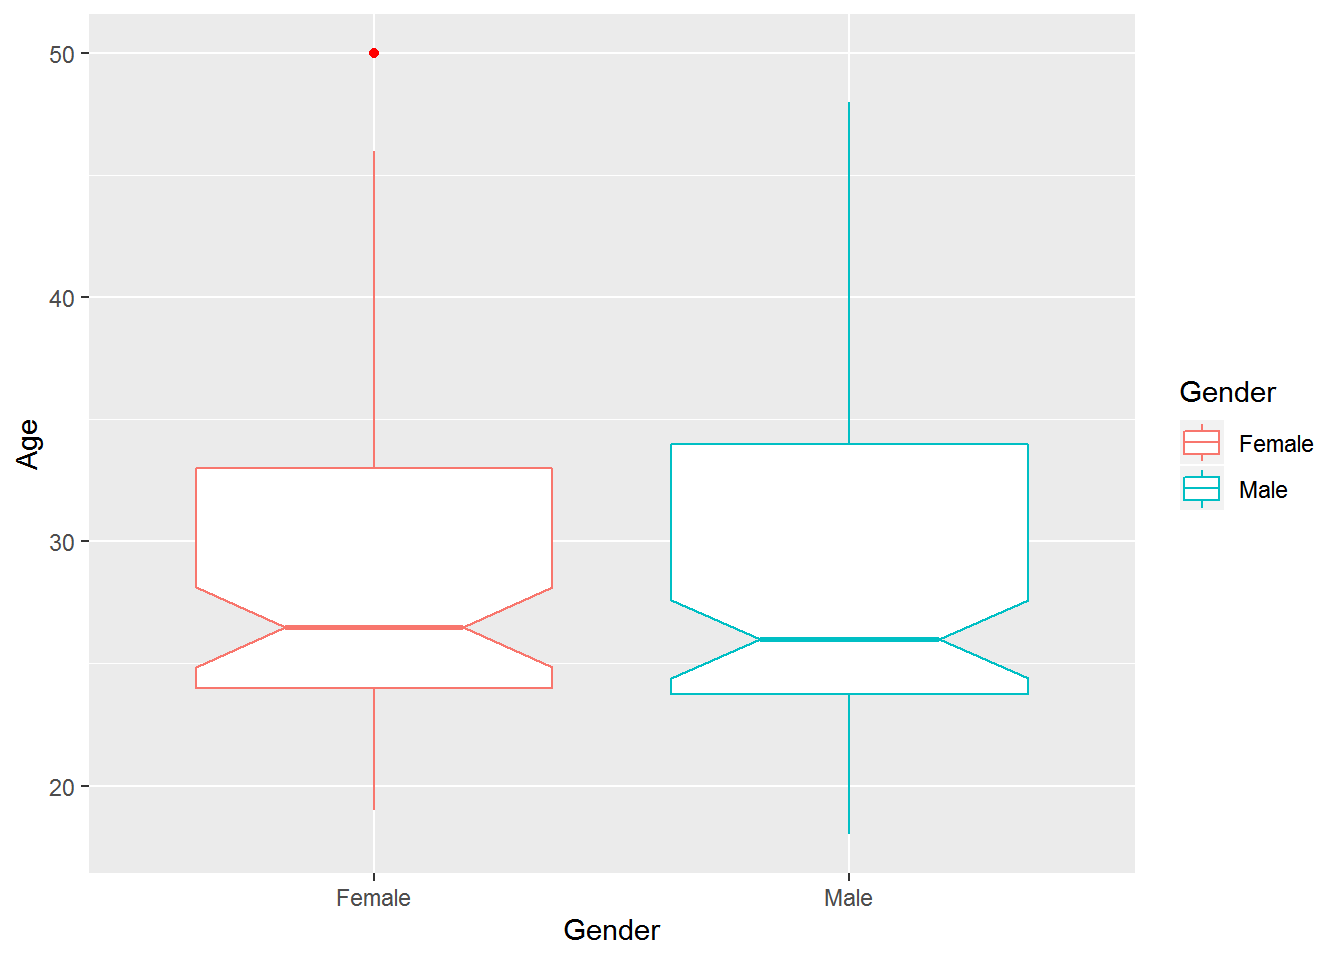
\includegraphics{index_files/figure-latex/unnamed-chunk-14-1.pdf}

this is biveriable / mean two veriable are used to show there relation
between them as per the statistical summary of the plot. its between
gender vs age. we find out female minimum age we have in this dataset is
19 and maximum is 50 as compare to female male has minimum 18 and
maximum 48.male data is more right skwed then female data.this
visualization telling us we have one outlier in female category age
50year is beyound the Q3+1.5IQR so we concider it outlier.

\#\#\#\#Age vs Product summary and plot

\begin{Shaded}
\begin{Highlighting}[]
\CommentTok{#statistical summary of Age and Product}
\KeywordTok{tapply}\NormalTok{(cardio_data}\OperatorTok{$}\NormalTok{Age,cardio_data}\OperatorTok{$}\NormalTok{Product,summary)}
\end{Highlighting}
\end{Shaded}

\begin{verbatim}
## $TM195
##    Min. 1st Qu.  Median    Mean 3rd Qu.    Max. 
##   18.00   23.00   26.00   28.55   33.00   50.00 
## 
## $TM498
##    Min. 1st Qu.  Median    Mean 3rd Qu.    Max. 
##   19.00   24.00   26.00   28.90   33.25   48.00 
## 
## $TM798
##    Min. 1st Qu.  Median    Mean 3rd Qu.    Max. 
##   22.00   24.75   27.00   29.10   30.25   48.00
\end{verbatim}

\begin{Shaded}
\begin{Highlighting}[]
\KeywordTok{ggplot}\NormalTok{(cardio_data,}\KeywordTok{aes}\NormalTok{(}\DataTypeTok{x=}\NormalTok{ Product,}\DataTypeTok{y=}\NormalTok{Age)) }\OperatorTok{+}\KeywordTok{geom_boxplot}\NormalTok{(}\KeywordTok{aes}\NormalTok{(}\DataTypeTok{colour =}\NormalTok{ Product), }\DataTypeTok{outlier.colour =} \StringTok{"red"}\NormalTok{,}\DataTypeTok{notch=}\OtherTok{FALSE}\NormalTok{) }
\end{Highlighting}
\end{Shaded}

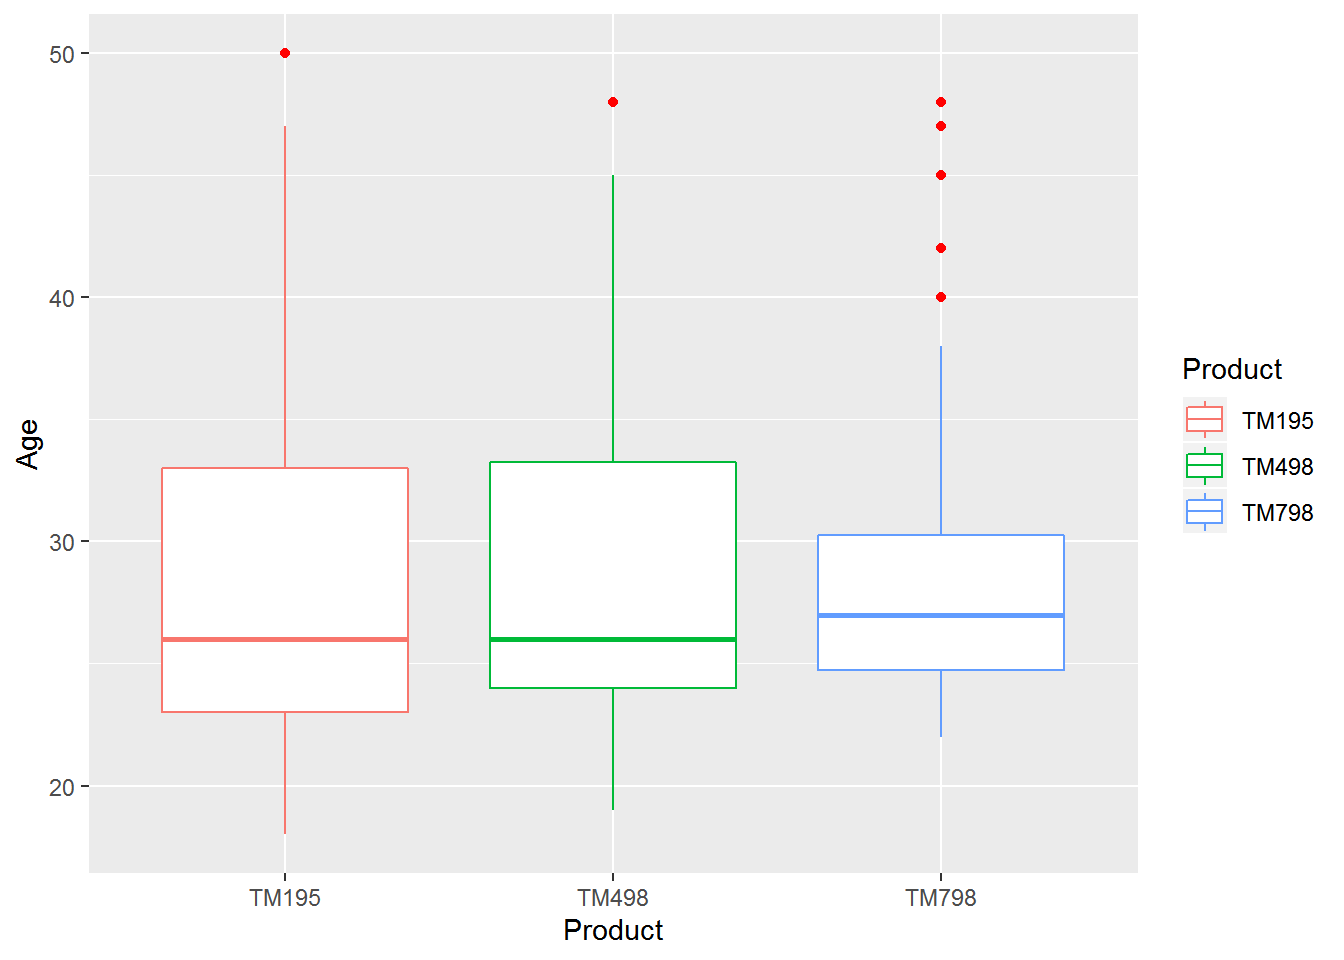
\includegraphics{index_files/figure-latex/unnamed-chunk-15-1.pdf}

In this figure we plot TM type and the user age. so here we will try to
find out what is the age group of people or how many people using each
paticular machine. As we see the statistical summary and graphical plot
TM195 is most popular TM type among user then Tm 498 then TM798
respectively. as we see Tm 195 users are min 18 to 46 year old, TM498
showing almost same resemblance but TM798 is only popular 22 to 37 years
old people using it. we also facing some outlier in this plot but most
of the outlier belong to TM798.

\hypertarget{gender-vs-fitness-summary-and-plot}{%
\paragraph{Gender vs Fitness summary and
plot}\label{gender-vs-fitness-summary-and-plot}}

\begin{Shaded}
\begin{Highlighting}[]
\CommentTok{#statistical summary of Age and Gender}
\NormalTok{cardio_data}\OperatorTok{$}\NormalTok{age_group <-}\StringTok{ }\KeywordTok{cut}\NormalTok{(cardio_data}\OperatorTok{$}\NormalTok{Age, }\DataTypeTok{breaks =} \KeywordTok{c}\NormalTok{(}\DecValTok{0}\NormalTok{, }\DecValTok{25}\NormalTok{, }\DecValTok{35}\NormalTok{, }\DecValTok{50}\NormalTok{), }
                             \DataTypeTok{labels =} \KeywordTok{c}\NormalTok{(}\StringTok{"less then 25"}\NormalTok{,}\StringTok{"25 to 35"}\NormalTok{,}\StringTok{"greater then 35"}\NormalTok{))}
\KeywordTok{tapply}\NormalTok{(cardio_data}\OperatorTok{$}\NormalTok{Fitness,cardio_data}\OperatorTok{$}\NormalTok{age_group,summary)}
\end{Highlighting}
\end{Shaded}

\begin{verbatim}
## $`less then 25`
##    Min. 1st Qu.  Median    Mean 3rd Qu.    Max. 
##   1.000   3.000   3.000   3.266   4.000   5.000 
## 
## $`25 to 35`
##    Min. 1st Qu.  Median    Mean 3rd Qu.    Max. 
##   1.000   3.000   3.000   3.329   4.000   5.000 
## 
## $`greater then 35`
##    Min. 1st Qu.  Median    Mean 3rd Qu.    Max. 
##   2.000   3.000   3.000   3.393   4.000   5.000
\end{verbatim}

\begin{Shaded}
\begin{Highlighting}[]
  \KeywordTok{ggplot}\NormalTok{(cardio_data,}\KeywordTok{aes}\NormalTok{(}\DataTypeTok{x=}\NormalTok{ age_group,}\DataTypeTok{y=}\NormalTok{Fitness)) }\OperatorTok{+}\KeywordTok{geom_point}\NormalTok{(}\KeywordTok{aes}\NormalTok{(}\DataTypeTok{col=}\NormalTok{Gender))}
\end{Highlighting}
\end{Shaded}

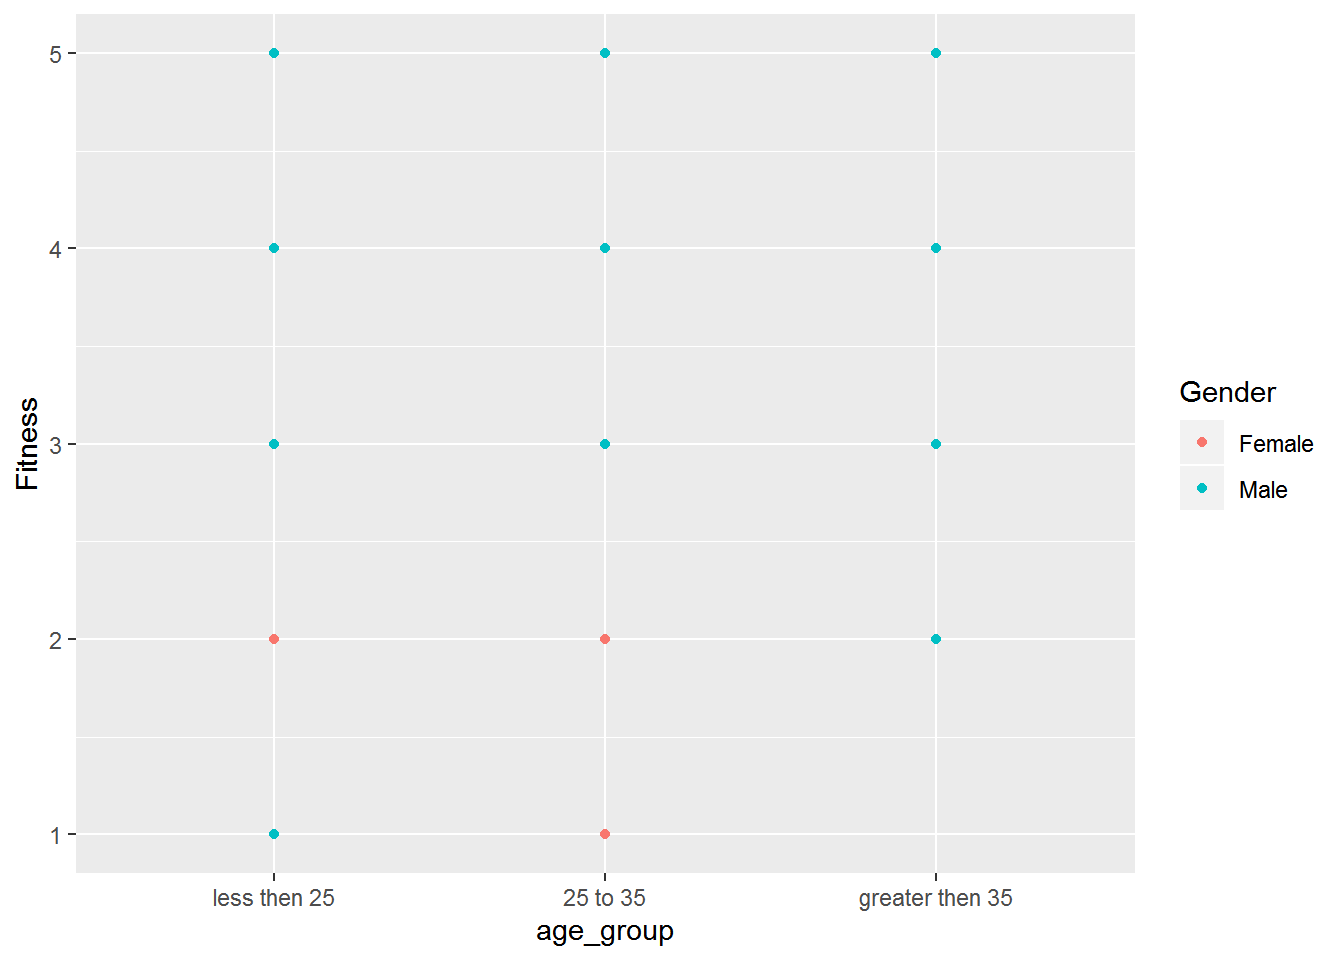
\includegraphics{index_files/figure-latex/unnamed-chunk-16-1.pdf}

we divided the age of the users into three age groups and then we check
the fitness lavel with the filter of Gender. fit of all we saw male are
more fit then female user as compare to age group no female user belong
to greater then 35 year old age group.

\hypertarget{tm-type-vs-user-income-summary-and-plot}{%
\paragraph{TM type vs User Income summary and
plot}\label{tm-type-vs-user-income-summary-and-plot}}

\begin{Shaded}
\begin{Highlighting}[]
\CommentTok{#statistical summary of income and product}
\KeywordTok{tapply}\NormalTok{(cardio_data}\OperatorTok{$}\NormalTok{Income,cardio_data}\OperatorTok{$}\NormalTok{Product,summary)}
\end{Highlighting}
\end{Shaded}

\begin{verbatim}
## $TM195
##    Min. 1st Qu.  Median    Mean 3rd Qu.    Max. 
##   29562   38658   46617   46418   53439   68220 
## 
## $TM498
##    Min. 1st Qu.  Median    Mean 3rd Qu.    Max. 
##   31836   44912   49460   48974   53439   67083 
## 
## $TM798
##    Min. 1st Qu.  Median    Mean 3rd Qu.    Max. 
##   48556   58205   76569   75442   90886  104581
\end{verbatim}

\begin{Shaded}
\begin{Highlighting}[]
\KeywordTok{ggplot}\NormalTok{(cardio_data,}\KeywordTok{aes}\NormalTok{(}\DataTypeTok{x=}\NormalTok{ Product,}\DataTypeTok{y=}\NormalTok{Income)) }\OperatorTok{+}\KeywordTok{geom_boxplot}\NormalTok{(}\KeywordTok{aes}\NormalTok{(}\DataTypeTok{colour =}\NormalTok{ Product), }\DataTypeTok{outlier.colour =} \StringTok{"red"}\NormalTok{,}\DataTypeTok{notch=}\OtherTok{FALSE}\NormalTok{) }\OperatorTok{+}\StringTok{ }\KeywordTok{scale_y_continuous}\NormalTok{(}\DataTypeTok{labels =}\NormalTok{ scales}\OperatorTok{::}\NormalTok{comma)}
\end{Highlighting}
\end{Shaded}

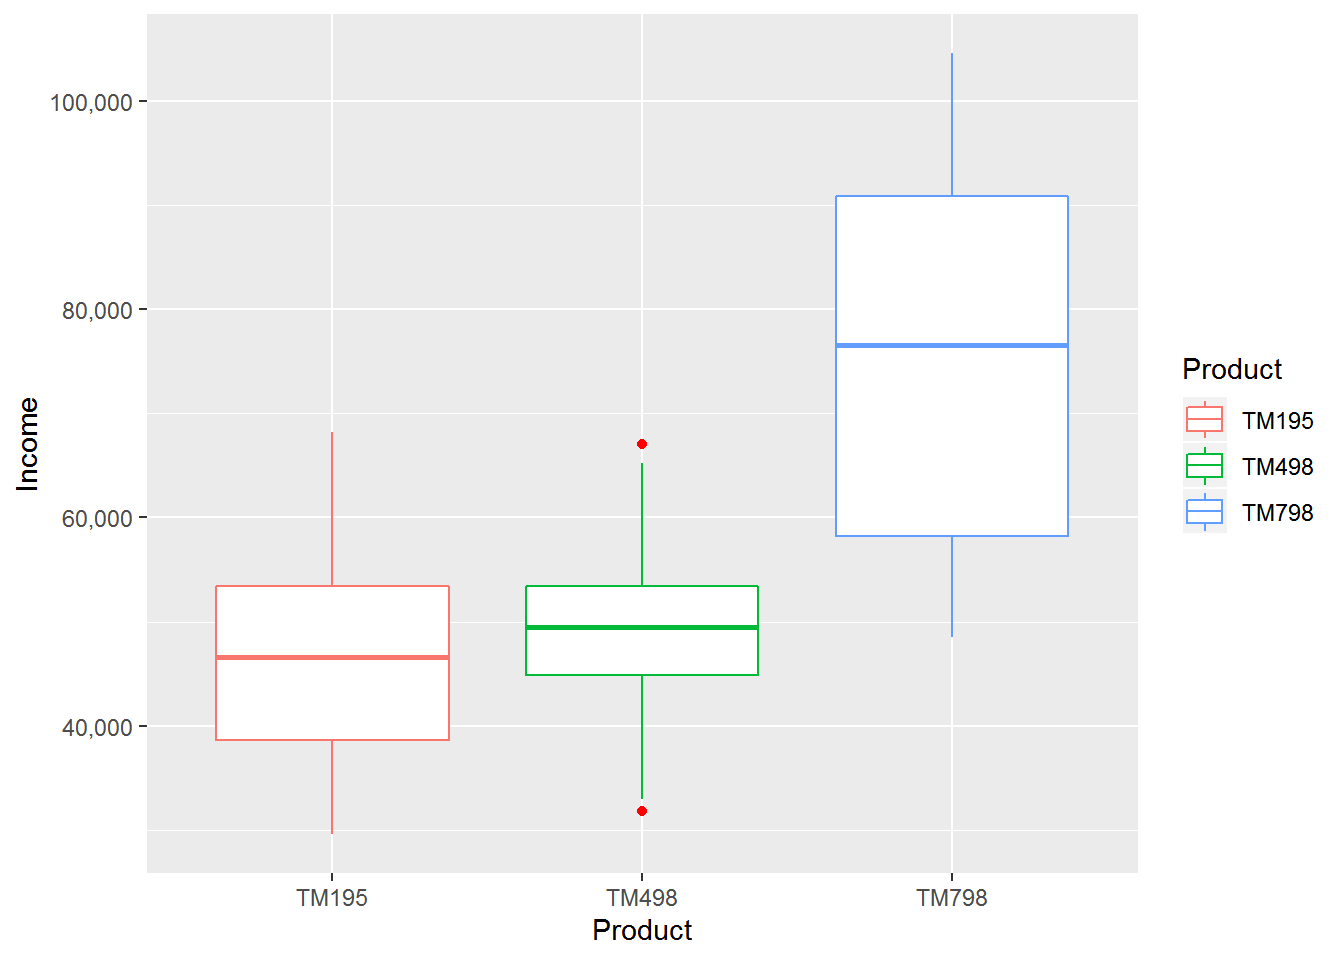
\includegraphics{index_files/figure-latex/unnamed-chunk-17-1.pdf}

In this plot we find out TM798 only hit the high income customer its
client has minimum 48 thousend and toward 1oo plus thousend. TM195
client has low salary as compared to other minimum 29 thousend to 68
thousend.

\hypertarget{product-vs-usage-summary-and-plot}{%
\paragraph{Product vs Usage summary and
plot}\label{product-vs-usage-summary-and-plot}}

\begin{Shaded}
\begin{Highlighting}[]
\CommentTok{#statistical summary of usage and product}
\KeywordTok{tapply}\NormalTok{(cardio_data}\OperatorTok{$}\NormalTok{Usage,cardio_data}\OperatorTok{$}\NormalTok{Product,summary)}
\end{Highlighting}
\end{Shaded}

\begin{verbatim}
## $TM195
##    Min. 1st Qu.  Median    Mean 3rd Qu.    Max. 
##   2.000   3.000   3.000   3.087   4.000   5.000 
## 
## $TM498
##    Min. 1st Qu.  Median    Mean 3rd Qu.    Max. 
##   2.000   3.000   3.000   3.067   3.250   5.000 
## 
## $TM798
##    Min. 1st Qu.  Median    Mean 3rd Qu.    Max. 
##   3.000   4.000   5.000   4.775   5.000   7.000
\end{verbatim}

\begin{Shaded}
\begin{Highlighting}[]
\KeywordTok{ggplot}\NormalTok{(cardio_data,}\KeywordTok{aes}\NormalTok{(}\DataTypeTok{x=}\NormalTok{ Product,}\DataTypeTok{y=}\NormalTok{Usage)) }\OperatorTok{+}\KeywordTok{geom_boxplot}\NormalTok{(}\KeywordTok{aes}\NormalTok{(}\DataTypeTok{fill =}\NormalTok{ Product), }\DataTypeTok{outlier.colour =} \StringTok{"red"}\NormalTok{,}\DataTypeTok{notch=}\OtherTok{FALSE}\NormalTok{) }\OperatorTok{+}\StringTok{ }\KeywordTok{scale_y_continuous}\NormalTok{(}\DataTypeTok{labels =}\NormalTok{ scales}\OperatorTok{::}\NormalTok{comma)}
\end{Highlighting}
\end{Shaded}

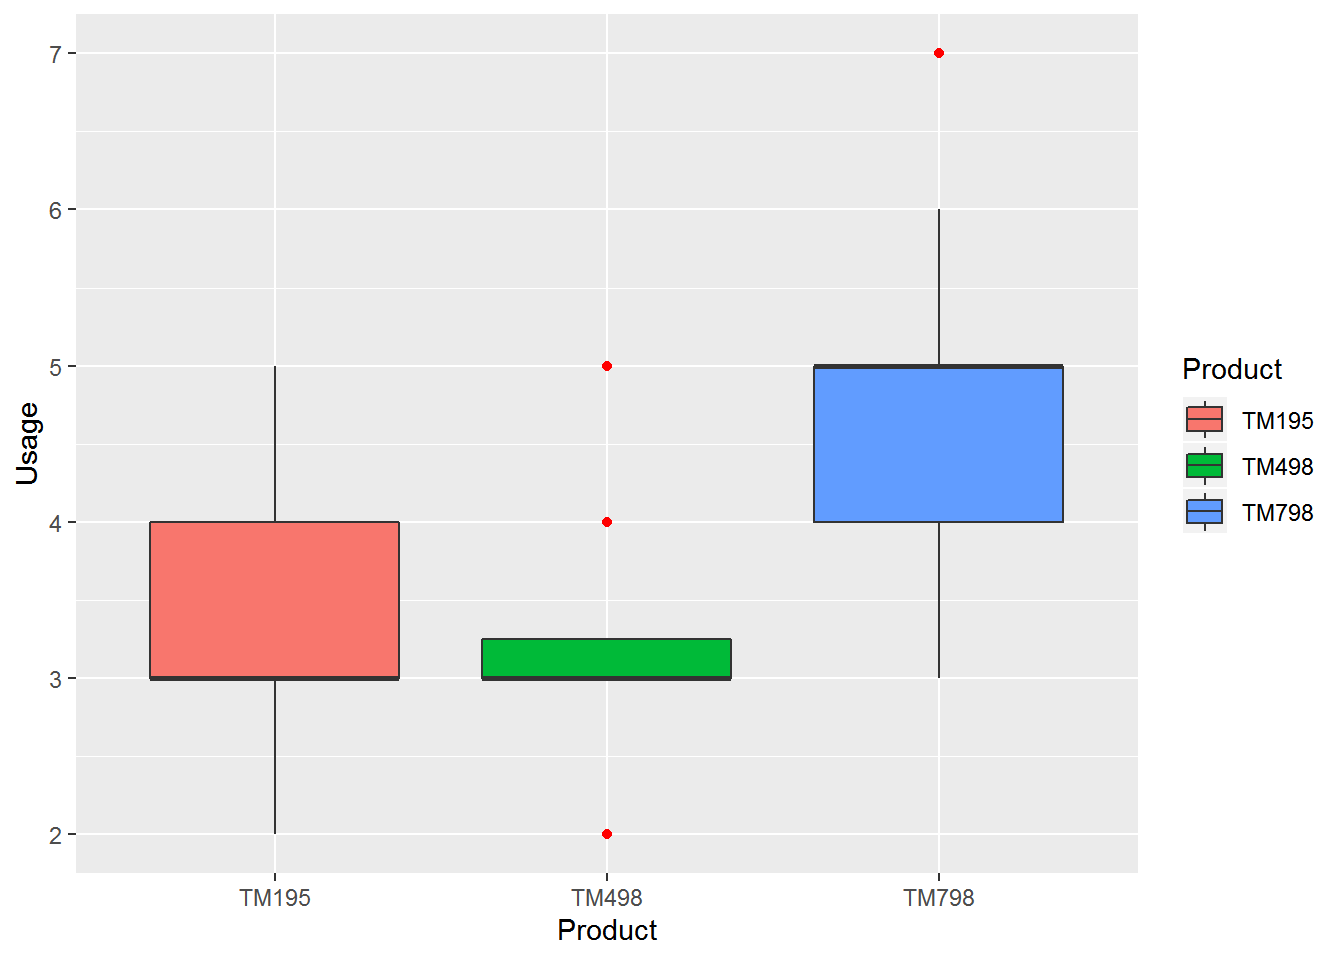
\includegraphics{index_files/figure-latex/unnamed-chunk-18-1.pdf}

in this plot we analyse TM798 usage is higher the other two products and
secound most using by the customer is TM195.

\hypertarget{usage-vs-income-summary-and-plot}{%
\paragraph{Usage vs Income summary and
plot}\label{usage-vs-income-summary-and-plot}}

\begin{Shaded}
\begin{Highlighting}[]
\CommentTok{#statistical summary of usge and income}
\KeywordTok{ggplot}\NormalTok{(cardio_data,}\KeywordTok{aes}\NormalTok{(}\DataTypeTok{x=}\KeywordTok{factor}\NormalTok{(Usage) ,}\DataTypeTok{y=}\NormalTok{Income)) }\OperatorTok{+}
\StringTok{  }\KeywordTok{geom_point}\NormalTok{(}\DataTypeTok{col=}\StringTok{"darkcyan"}\NormalTok{)}\OperatorTok{+}
\StringTok{  }\KeywordTok{geom_smooth}\NormalTok{(}\DataTypeTok{method =} \StringTok{"lm"}\NormalTok{, }\DataTypeTok{se =} \OtherTok{FALSE}\NormalTok{)}\OperatorTok{+}
\StringTok{  }\KeywordTok{scale_y_continuous}\NormalTok{(}\DataTypeTok{labels =}\NormalTok{scales}\OperatorTok{::}\NormalTok{comma)}\OperatorTok{+}
\StringTok{  }\KeywordTok{facet_wrap}\NormalTok{(}\OperatorTok{~}\StringTok{ }\NormalTok{Gender)}
\end{Highlighting}
\end{Shaded}

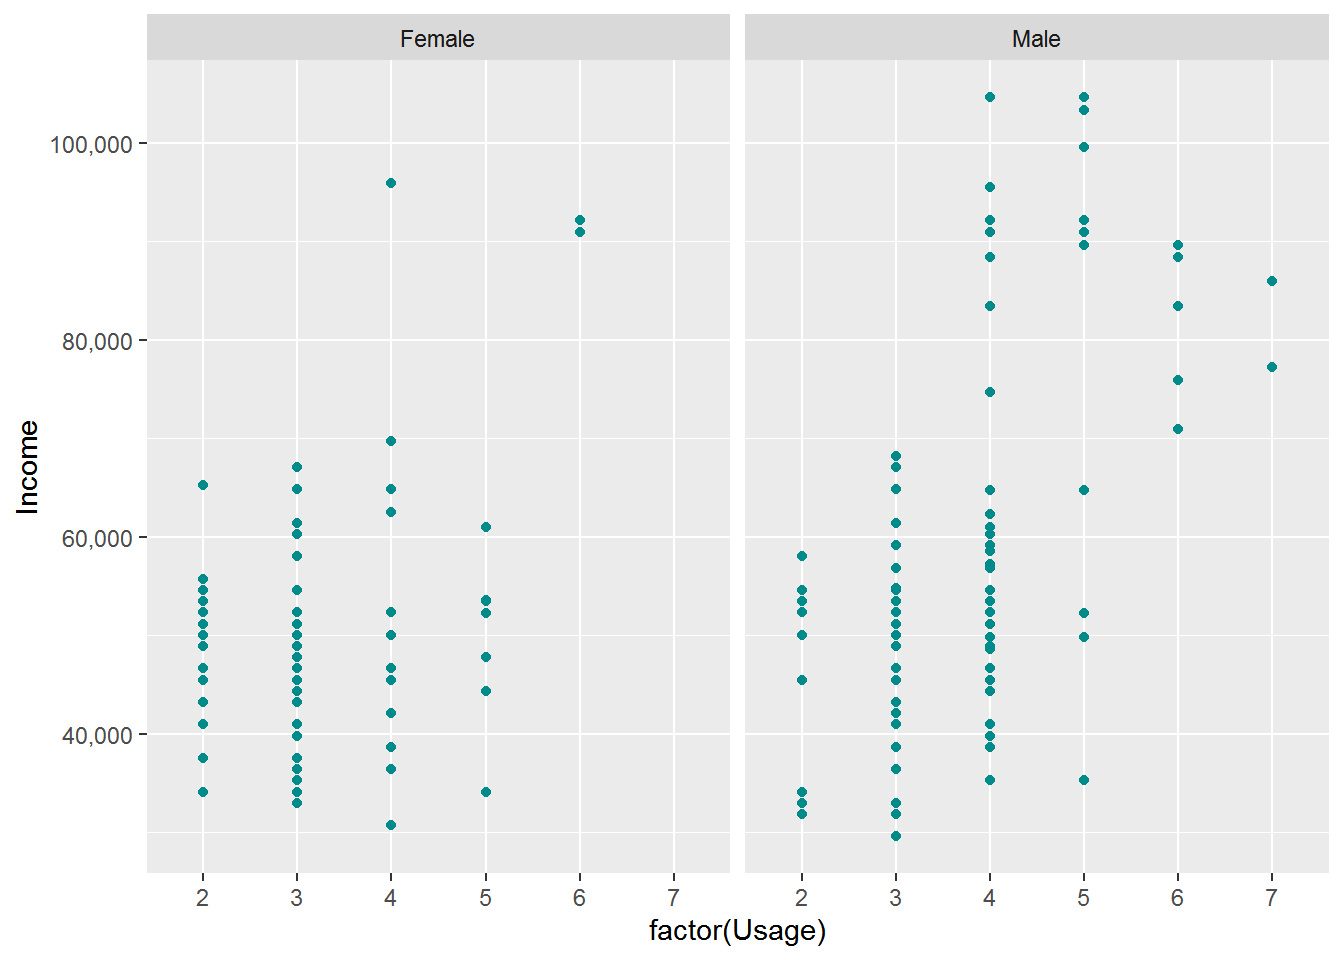
\includegraphics{index_files/figure-latex/unnamed-chunk-19-1.pdf}

In this we analyse usage of the treadmill and the customer income has
relation between then we saw when ever the income increase the usage of
the product also increase.

\begin{Shaded}
\begin{Highlighting}[]
\KeywordTok{tapply}\NormalTok{(cardio_data}\OperatorTok{$}\NormalTok{Fitness,cardio_data}\OperatorTok{$}\NormalTok{Product,summary)}
\end{Highlighting}
\end{Shaded}

\begin{verbatim}
## $TM195
##    Min. 1st Qu.  Median    Mean 3rd Qu.    Max. 
##   1.000   3.000   3.000   2.962   3.000   5.000 
## 
## $TM498
##    Min. 1st Qu.  Median    Mean 3rd Qu.    Max. 
##     1.0     3.0     3.0     2.9     3.0     4.0 
## 
## $TM798
##    Min. 1st Qu.  Median    Mean 3rd Qu.    Max. 
##   3.000   4.000   5.000   4.625   5.000   5.000
\end{verbatim}

\begin{Shaded}
\begin{Highlighting}[]
\KeywordTok{ggplot}\NormalTok{(cardio_data,}\KeywordTok{aes}\NormalTok{(}\DataTypeTok{x=}\NormalTok{ Product,}\DataTypeTok{y=}\NormalTok{Fitness)) }\OperatorTok{+}\KeywordTok{geom_boxplot}\NormalTok{(}\KeywordTok{aes}\NormalTok{(}\DataTypeTok{fill =}\NormalTok{ Product), }\DataTypeTok{outlier.colour =} \StringTok{"red"}\NormalTok{,}\DataTypeTok{notch=}\OtherTok{FALSE}\NormalTok{) }\OperatorTok{+}\StringTok{ }\KeywordTok{scale_y_continuous}\NormalTok{(}\DataTypeTok{labels =}\NormalTok{ scales}\OperatorTok{::}\NormalTok{comma)}
\end{Highlighting}
\end{Shaded}

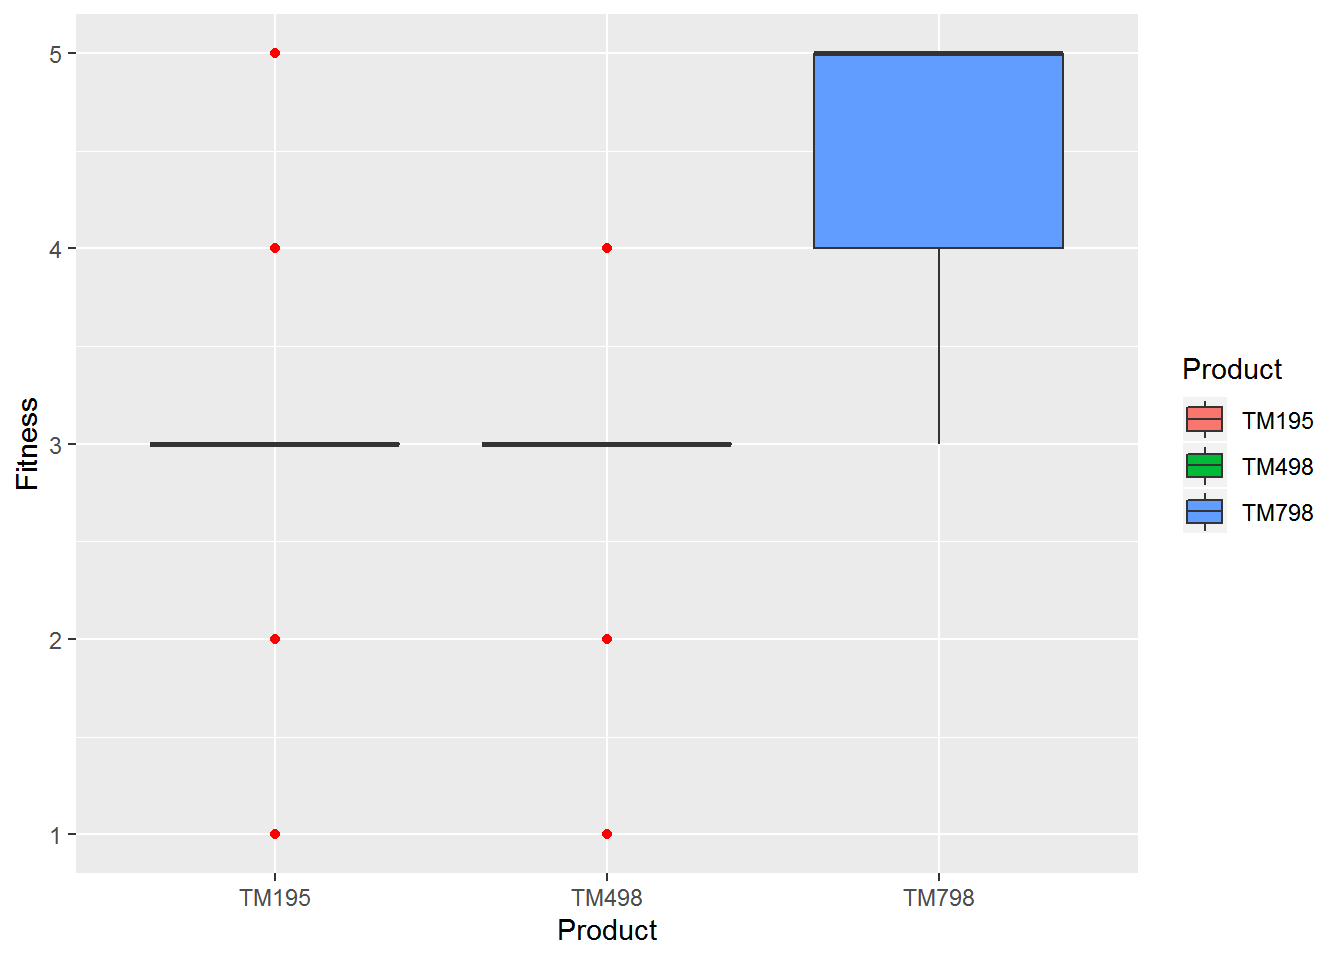
\includegraphics{index_files/figure-latex/unnamed-chunk-20-1.pdf}

\hypertarget{correlation-plot}{%
\paragraph{correlation Plot}\label{correlation-plot}}

\begin{Shaded}
\begin{Highlighting}[]
\KeywordTok{corrplot}\NormalTok{(}\KeywordTok{cor}\NormalTok{(cardio_data[,}\DecValTok{6}\OperatorTok{:}\DecValTok{9}\NormalTok{]))}
\end{Highlighting}
\end{Shaded}

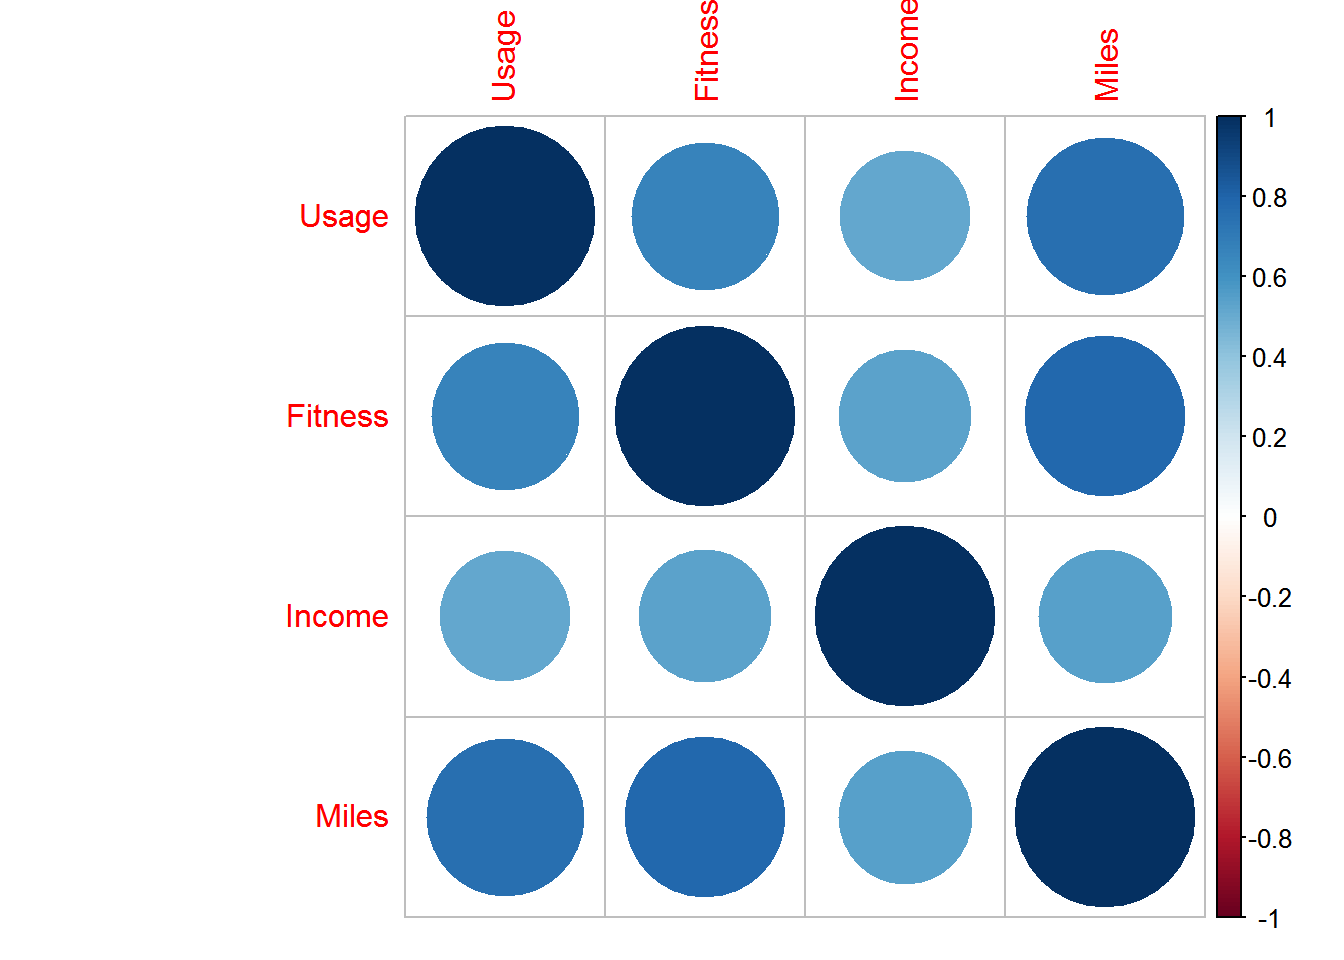
\includegraphics{index_files/figure-latex/unnamed-chunk-21-1.pdf}

we draw correlation graph amoung numeric veriables and we find out great
positive correlation amoung all of them.

\hypertarget{fitness-vs-miles-summary-and-plot}{%
\paragraph{Fitness Vs Miles summary and
plot}\label{fitness-vs-miles-summary-and-plot}}

\begin{Shaded}
\begin{Highlighting}[]
\CommentTok{#statistical summary of miles and fitness}
\NormalTok{z <-}\StringTok{ }\KeywordTok{lm}\NormalTok{(Fitness }\OperatorTok{~}\StringTok{ }\NormalTok{Miles, }\DataTypeTok{data =}\NormalTok{ cardio_data)}
\KeywordTok{coef}\NormalTok{(z)}
\end{Highlighting}
\end{Shaded}

\begin{verbatim}
## (Intercept)       Miles 
##  1.81208079  0.01452627
\end{verbatim}

\begin{Shaded}
\begin{Highlighting}[]
\KeywordTok{tapply}\NormalTok{(cardio_data}\OperatorTok{$}\NormalTok{Miles,cardio_data}\OperatorTok{$}\NormalTok{Fitness,summary)}
\end{Highlighting}
\end{Shaded}

\begin{verbatim}
## $`1`
##    Min. 1st Qu.  Median    Mean 3rd Qu.    Max. 
##    21.0    27.5    34.0    34.0    40.5    47.0 
## 
## $`2`
##    Min. 1st Qu.  Median    Mean 3rd Qu.    Max. 
##   38.00   43.25   47.00   51.69   53.00   85.00 
## 
## $`3`
##    Min. 1st Qu.  Median    Mean 3rd Qu.    Max. 
##   53.00   75.00   85.00   87.19   95.00  170.00 
## 
## $`4`
##    Min. 1st Qu.  Median    Mean 3rd Qu.    Max. 
##    74.0   106.0   127.0   131.6   160.0   212.0 
## 
## $`5`
##    Min. 1st Qu.  Median    Mean 3rd Qu.    Max. 
##    80.0   150.0   170.0   178.9   200.0   360.0
\end{verbatim}

\begin{Shaded}
\begin{Highlighting}[]
\KeywordTok{ggplot}\NormalTok{(cardio_data,}\KeywordTok{aes}\NormalTok{(}\DataTypeTok{x=}\KeywordTok{factor}\NormalTok{(Fitness),}\DataTypeTok{y=}\NormalTok{Miles)) }\OperatorTok{+}
\StringTok{  }\KeywordTok{geom_point}\NormalTok{(}\KeywordTok{aes}\NormalTok{(}\DataTypeTok{shape=}\KeywordTok{factor}\NormalTok{(MaritalStatus),}\DataTypeTok{col=}\KeywordTok{factor}\NormalTok{(MaritalStatus)))}\OperatorTok{+}
\StringTok{  }\KeywordTok{geom_smooth}\NormalTok{(}\DataTypeTok{method =} \StringTok{"lm"}\NormalTok{, }\DataTypeTok{se =} \OtherTok{FALSE}\NormalTok{)}
\end{Highlighting}
\end{Shaded}

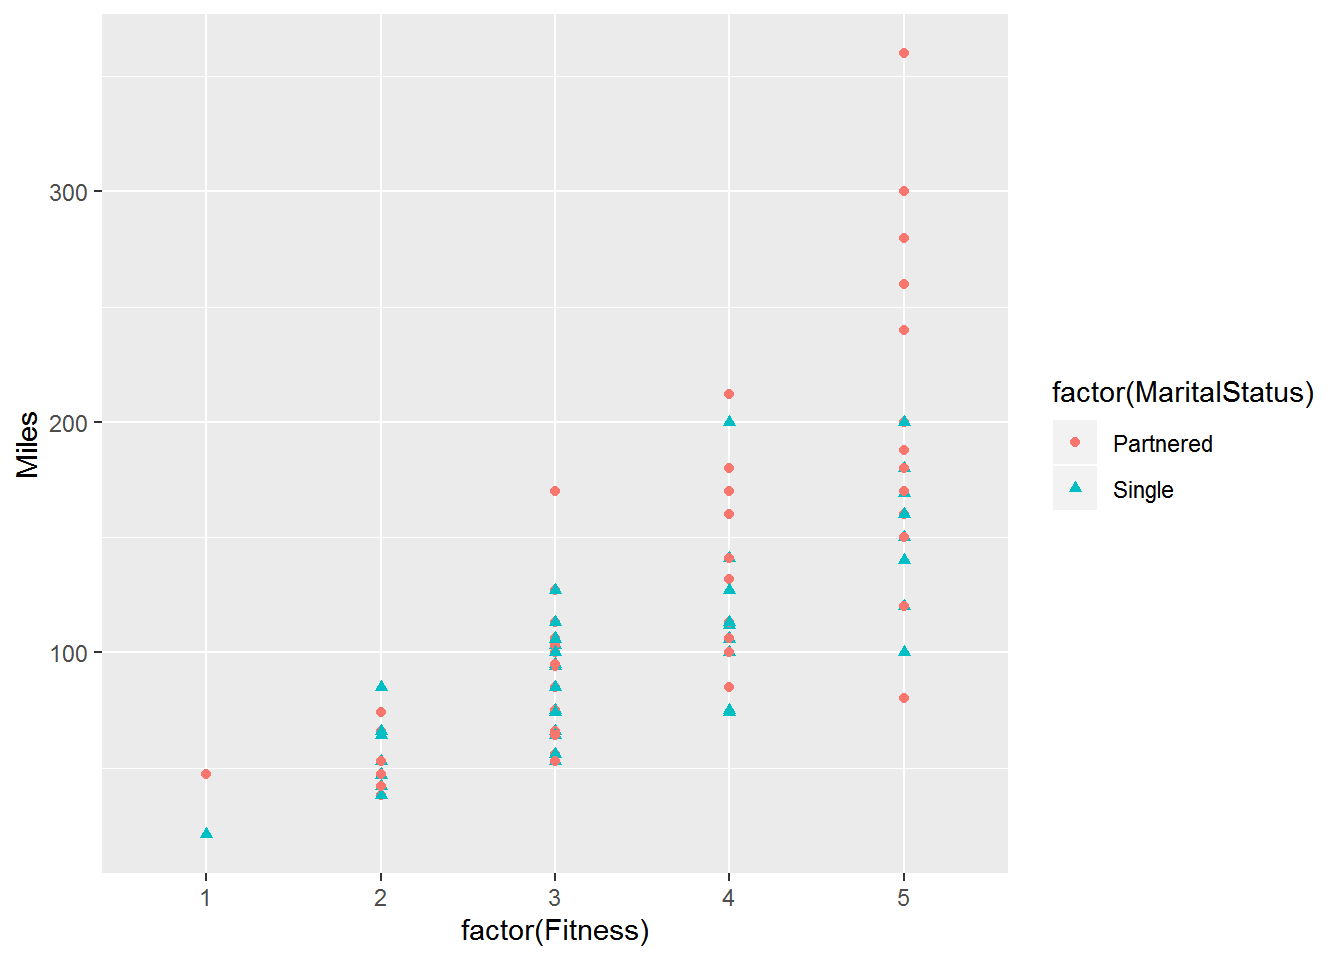
\includegraphics{index_files/figure-latex/unnamed-chunk-22-1.pdf}

\begin{Shaded}
\begin{Highlighting}[]
  \CommentTok{#geom_abline(intercept = 1.81, slope = 0.01)}
\end{Highlighting}
\end{Shaded}

here we noticed fitness increase with respect to miles increase its
shows us positive correlation and we filter it with Marital status. we
saw customer who has partnered has more fit and more miles cover as
respect to who are single.

\hypertarget{fitness-vs-usage}{%
\paragraph{Fitness vs usage}\label{fitness-vs-usage}}

\begin{Shaded}
\begin{Highlighting}[]
\KeywordTok{plot}\NormalTok{(}\KeywordTok{aggregate}\NormalTok{(Fitness}\OperatorTok{~}\NormalTok{Usage,}\DataTypeTok{data=}\NormalTok{ cardio_data,mean),}\DataTypeTok{type =} \StringTok{"b"}\NormalTok{,}\DataTypeTok{main=}\StringTok{"Fitness vs usage"}\NormalTok{,}\DataTypeTok{col=}\StringTok{"darkcyan"}\NormalTok{)}
\end{Highlighting}
\end{Shaded}

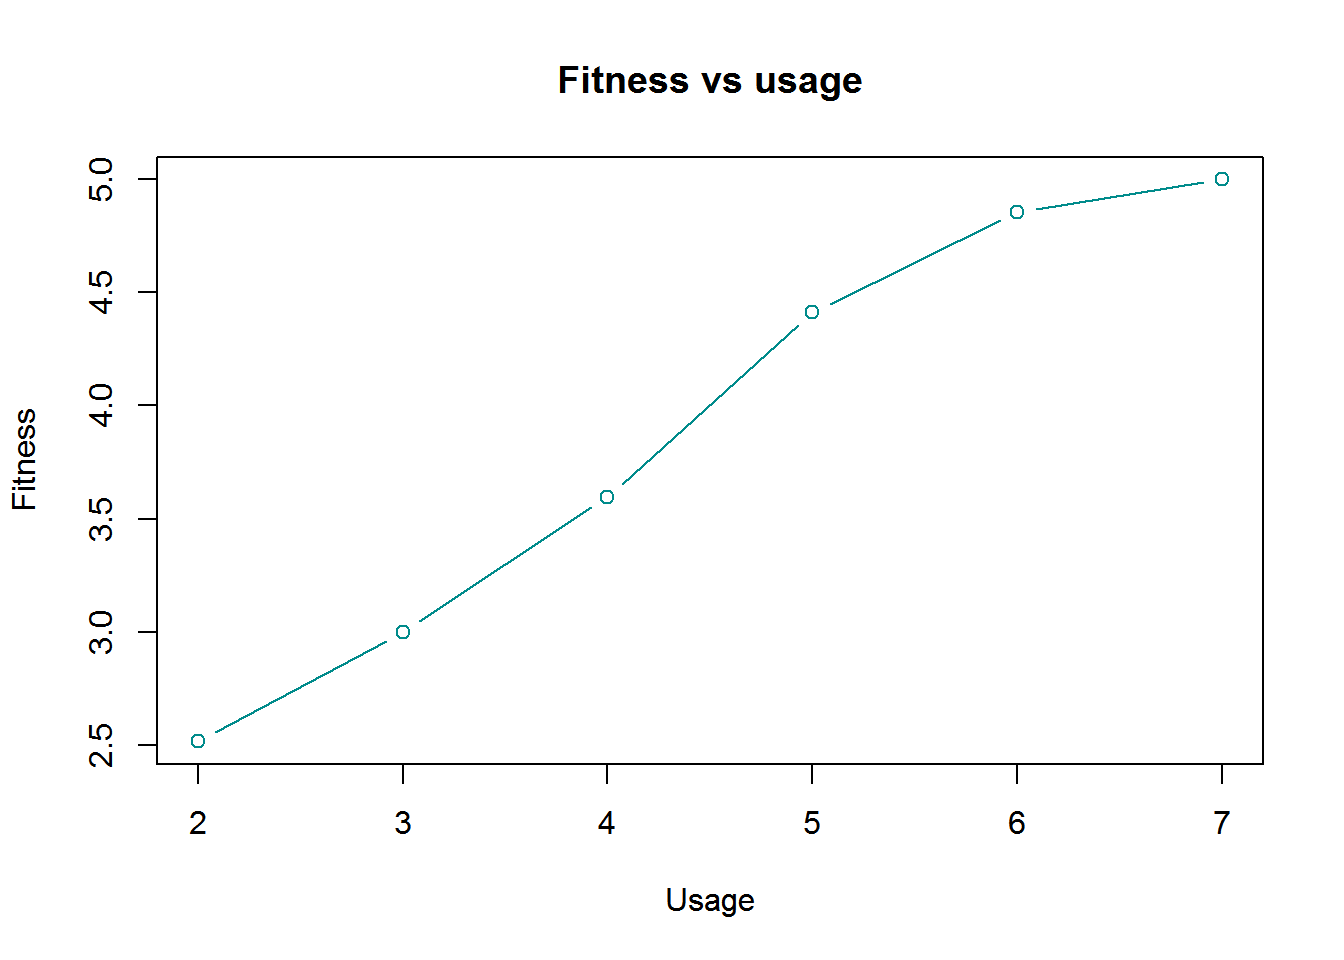
\includegraphics{index_files/figure-latex/unnamed-chunk-23-1.pdf}

we noticed fitness and usage has positive correlation.

\hypertarget{age-vs-income-plot}{%
\paragraph{Age vs Income plot}\label{age-vs-income-plot}}

\begin{Shaded}
\begin{Highlighting}[]
\KeywordTok{ggplot}\NormalTok{(cardio_data,}\KeywordTok{aes}\NormalTok{(}\DataTypeTok{x=}\NormalTok{Age ,}\DataTypeTok{y=}\NormalTok{Income)) }\OperatorTok{+}
\StringTok{  }\KeywordTok{geom_point}\NormalTok{(}\DataTypeTok{col=}\StringTok{"darkcyan"}\NormalTok{)}\OperatorTok{+}
\StringTok{  }\KeywordTok{scale_y_continuous}\NormalTok{(}\DataTypeTok{labels =}\NormalTok{scales}\OperatorTok{::}\NormalTok{comma)}\OperatorTok{+}
\StringTok{  }\KeywordTok{facet_wrap}\NormalTok{(}\OperatorTok{~}\StringTok{ }\NormalTok{Gender)}\OperatorTok{+}
\StringTok{  }\KeywordTok{geom_smooth}\NormalTok{(}\DataTypeTok{method =} \StringTok{"lm"}\NormalTok{, }\DataTypeTok{se =} \OtherTok{FALSE}\NormalTok{)}\OperatorTok{+}
\StringTok{  }\KeywordTok{theme}\NormalTok{(}\DataTypeTok{strip.background =} \KeywordTok{element_rect}\NormalTok{(}\DataTypeTok{fill=}\KeywordTok{c}\NormalTok{(}\StringTok{"darkcyan"}\NormalTok{)))}\OperatorTok{+}
\StringTok{  }\KeywordTok{ggtitle}\NormalTok{(}\StringTok{"Age vs Income Plot "}\NormalTok{)}
\end{Highlighting}
\end{Shaded}

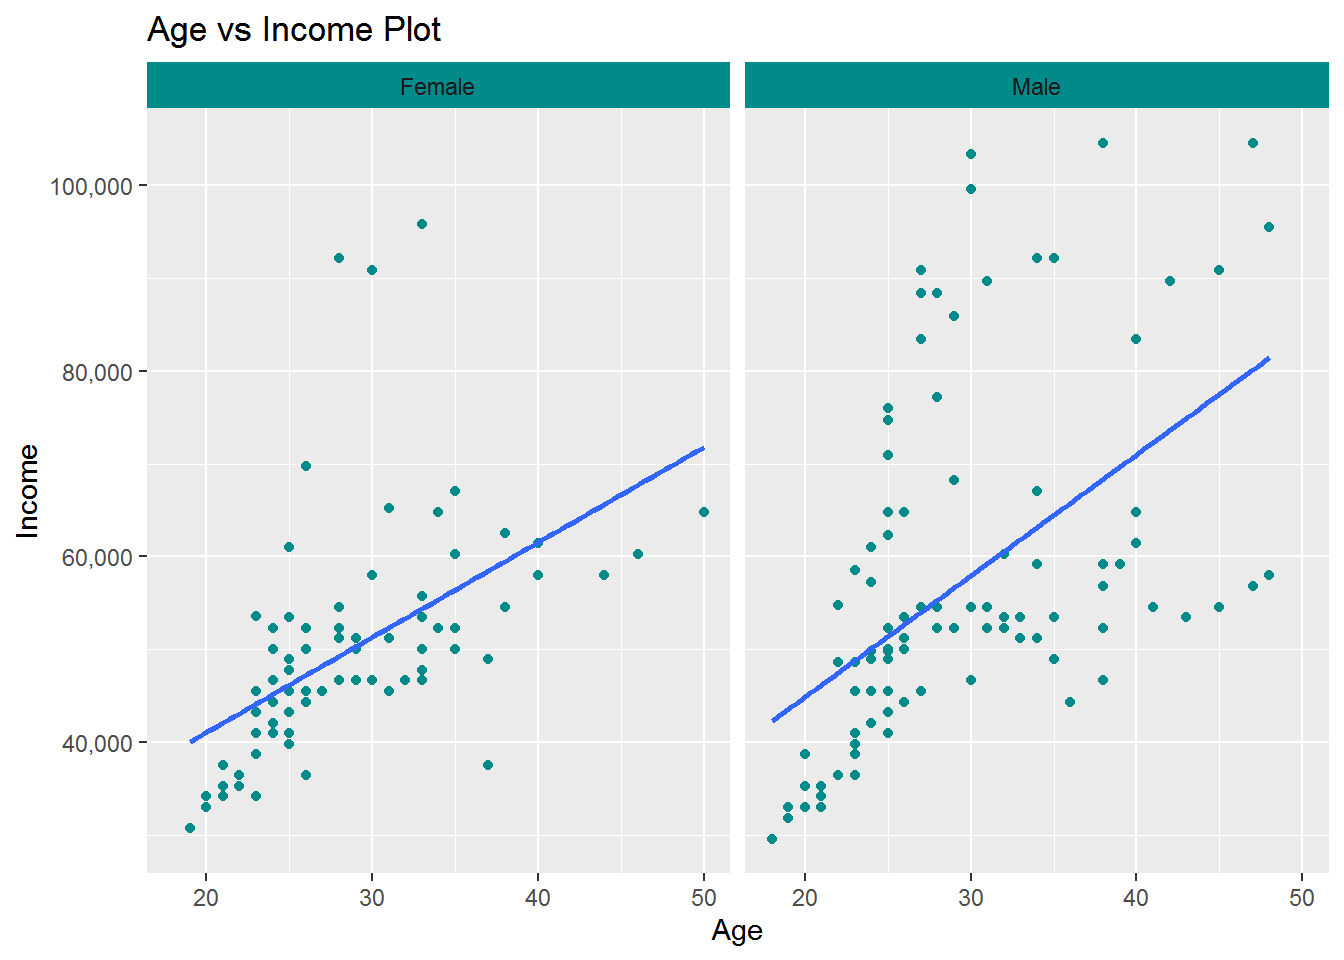
\includegraphics{index_files/figure-latex/unnamed-chunk-24-1.pdf}

we saw some positive correlation between age and income with repect to
gender. we also find out the slope of the line in male panel is higher
then female panel its mean male age and income has more stronger
correlation between them as respect to female.

\hypertarget{education-vs-income-plot}{%
\paragraph{Education vs Income Plot}\label{education-vs-income-plot}}

\begin{Shaded}
\begin{Highlighting}[]
\KeywordTok{ggplot}\NormalTok{(cardio_data,}\KeywordTok{aes}\NormalTok{(}\DataTypeTok{x=}\NormalTok{Education ,}\DataTypeTok{y=}\NormalTok{Income)) }\OperatorTok{+}
\StringTok{  }\KeywordTok{geom_point}\NormalTok{(}\DataTypeTok{col=}\StringTok{"darkcyan"}\NormalTok{)}\OperatorTok{+}
\StringTok{  }\KeywordTok{scale_y_continuous}\NormalTok{(}\DataTypeTok{labels =}\NormalTok{scales}\OperatorTok{::}\NormalTok{comma)}\OperatorTok{+}
\StringTok{  }\KeywordTok{facet_wrap}\NormalTok{(}\OperatorTok{~}\StringTok{ }\NormalTok{Gender)}\OperatorTok{+}
\StringTok{  }\KeywordTok{geom_smooth}\NormalTok{(}\DataTypeTok{method =} \StringTok{"lm"}\NormalTok{, }\DataTypeTok{se =} \OtherTok{FALSE}\NormalTok{)}\OperatorTok{+}
\StringTok{  }\KeywordTok{theme}\NormalTok{(}\DataTypeTok{strip.background =} \KeywordTok{element_rect}\NormalTok{(}\DataTypeTok{fill=}\KeywordTok{c}\NormalTok{(}\StringTok{"darkcyan"}\NormalTok{)))}\OperatorTok{+}
\StringTok{  }\KeywordTok{ggtitle}\NormalTok{(}\StringTok{"Education vs Income Plot "}\NormalTok{)}
\end{Highlighting}
\end{Shaded}

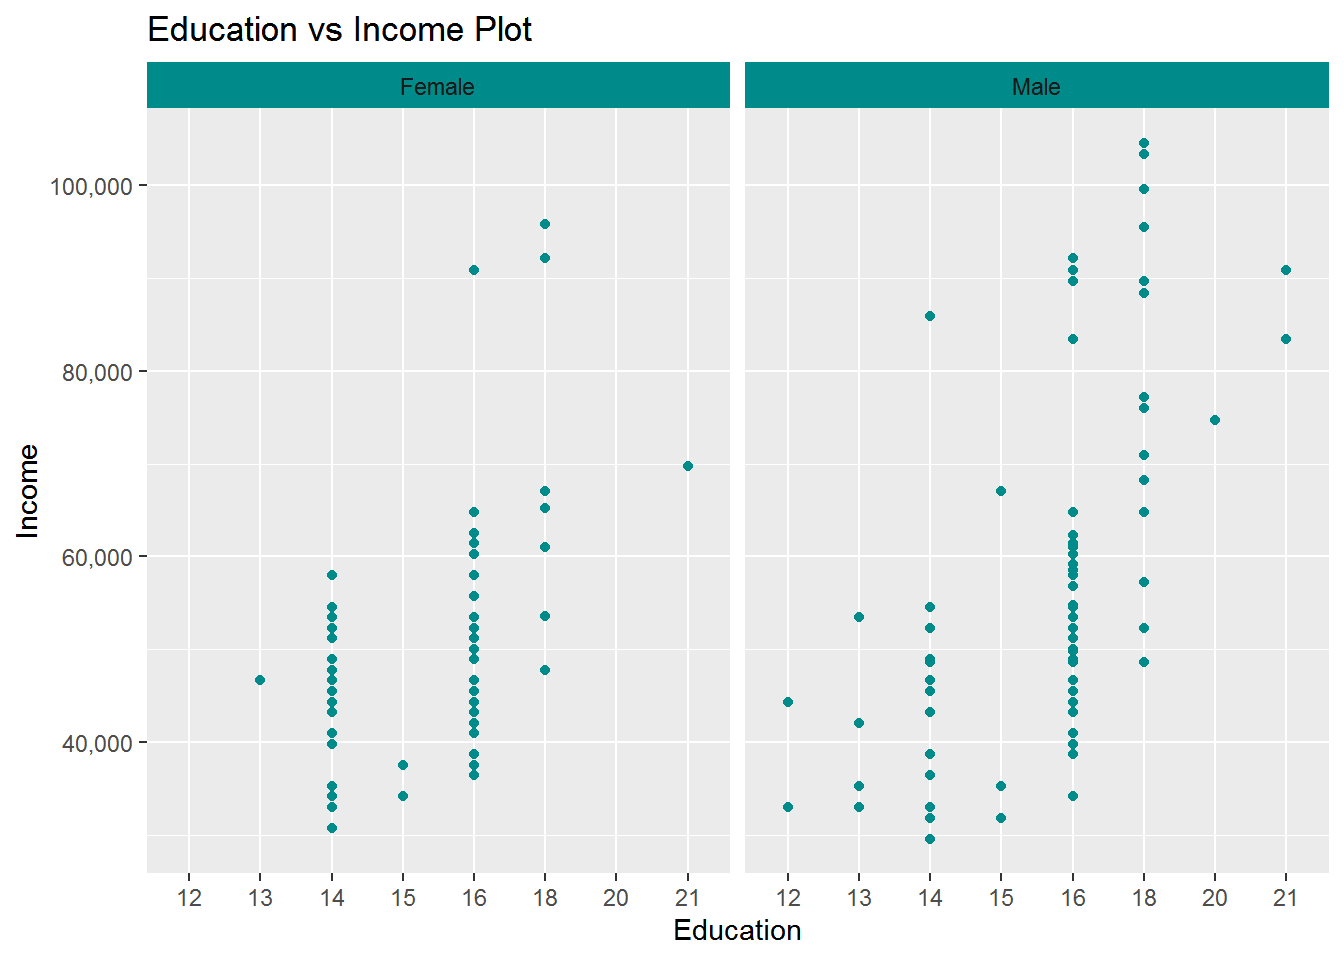
\includegraphics{index_files/figure-latex/unnamed-chunk-25-1.pdf}

Education and income also has positive correlation with respect to
gender.graph showing us male are getting higher salary then female
because the slope of the line is higher in male graph.

\hypertarget{age-vs-miles}{%
\paragraph{AGE Vs Miles}\label{age-vs-miles}}

\begin{Shaded}
\begin{Highlighting}[]
\KeywordTok{ggplot}\NormalTok{(cardio_data,}\KeywordTok{aes}\NormalTok{(}\DataTypeTok{x=}\NormalTok{Age ,}\DataTypeTok{y=}\NormalTok{Miles)) }\OperatorTok{+}
\StringTok{  }\KeywordTok{geom_point}\NormalTok{(}\DataTypeTok{col=}\StringTok{"darkcyan"}\NormalTok{)}\OperatorTok{+}
\StringTok{  }\KeywordTok{scale_y_continuous}\NormalTok{(}\DataTypeTok{labels =}\NormalTok{scales}\OperatorTok{::}\NormalTok{comma)}\OperatorTok{+}
\StringTok{  }\KeywordTok{facet_wrap}\NormalTok{(}\OperatorTok{~}\StringTok{ }\NormalTok{Gender)}\OperatorTok{+}
\StringTok{  }\KeywordTok{geom_smooth}\NormalTok{(}\DataTypeTok{method =} \StringTok{"lm"}\NormalTok{, }\DataTypeTok{se =} \OtherTok{FALSE}\NormalTok{)}\OperatorTok{+}
\StringTok{  }\KeywordTok{theme}\NormalTok{(}\DataTypeTok{strip.background =} \KeywordTok{element_rect}\NormalTok{(}\DataTypeTok{fill=}\KeywordTok{c}\NormalTok{(}\StringTok{"darkcyan"}\NormalTok{)))}\OperatorTok{+}
\StringTok{  }\KeywordTok{ggtitle}\NormalTok{(}\StringTok{"AGE Vs Miles"}\NormalTok{)}
\end{Highlighting}
\end{Shaded}

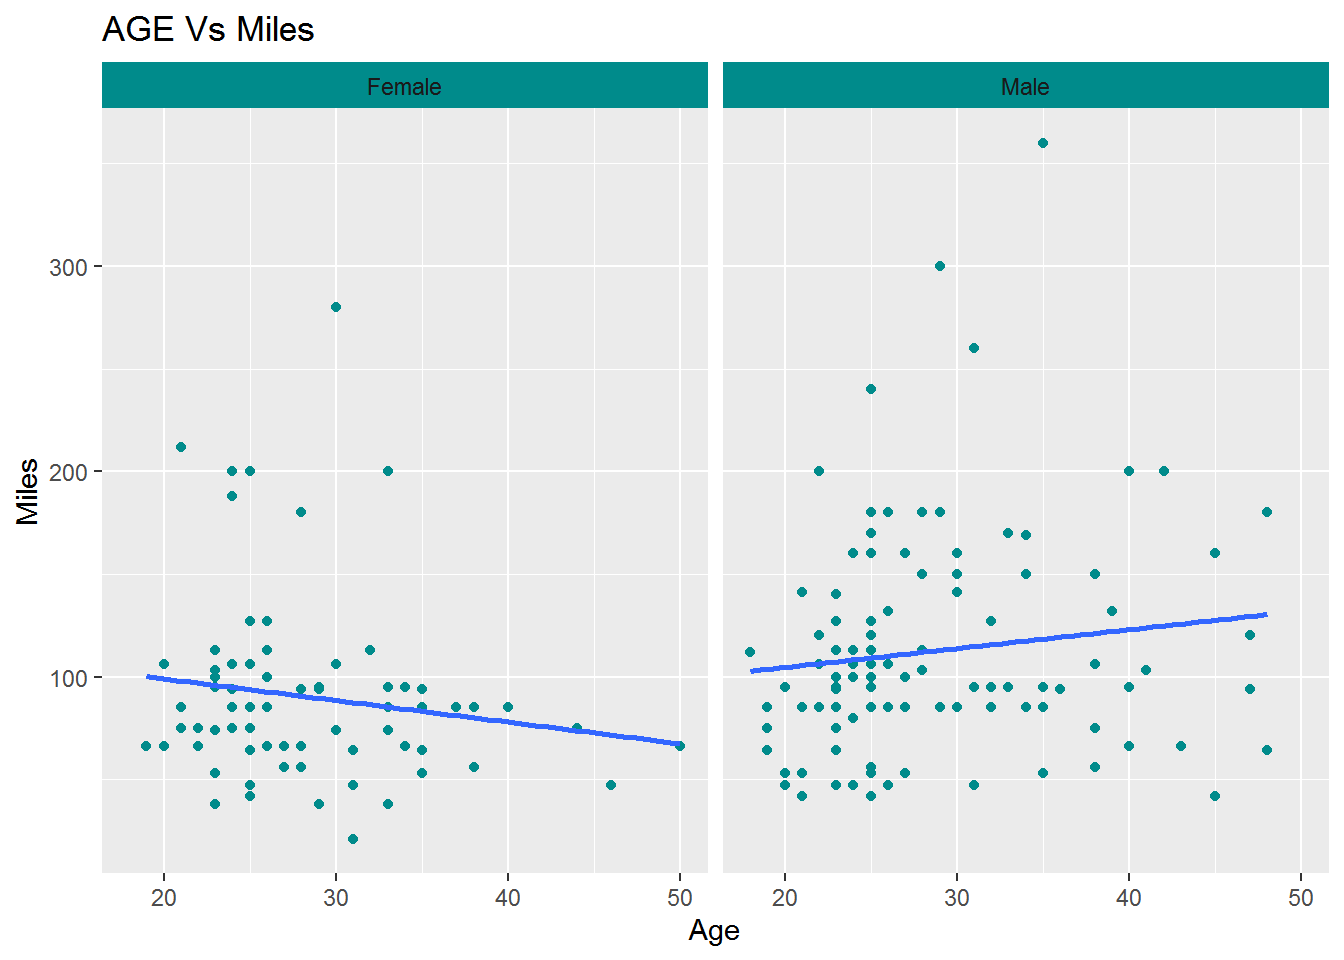
\includegraphics{index_files/figure-latex/unnamed-chunk-26-1.pdf}

here we saw some interesting ehaviour male has positive
coorrelationbetween age and miles its mean male customers are covering
miles increase with respect to age. But female has negative correlation
between age and miles covering.

\hypertarget{conclusion}{%
\subsubsection{Conclusion}\label{conclusion}}

The data shows prodct TM195 is most popular ine AGE group and on weekly
usage basis but product TM195 target only 29 thousend to 70 thousend
income customer but with respect to this product TM 798 target much
higher range of thecustomer.Product TM798 also gives showing us a good
result in weekly useage.But Product TM498 is showing us the negetive
correlation in usage and Income sides. This data also shows us when we
increase the weekly use we increse the miles and also we increase the
fitness rate. this data shows us the customers who has partenerd
spending more time and more fit then those who are single. This data
tells us male are getting paid more then female customers and female
customers reduce the mile with respect to age.

for the company interest when the company design the new product company
has to take attention on female users because female users health
condiction is worst then male users. upon the this interest we have to
design the product where female users build an interest init and also
concider the female users income codition.

\#\#*************THE END *************

\end{document}
